\chapter{Functions}
\setcounter{figure}{0}
\setcounter{subfigure}{0}

Functions are mathematical building blocks for designing machines, predicting natural disasters, curing diseases, understanding world economies and for keeping aeroplanes in the air. Functions can take input from many variables, but always give the same answer, unique to that function. It is the fact that you always get the same answer from a set of inputs that makes functions special.\par 
A major advantage of functions is that they allow us to visualise equations in terms of a graph. A graph is an accurate drawing of a function and is much easier to read than lists of numbers. In this chapter we will learn how to understand and create real valued functions, how to read graphs and how to draw them.\par 
In addition to their use in the problems facing humanity, functions also appear on a day-to-day level, so they are worth learning about. A function is always dependent on one or more variables, like time, distance or a more abstract quantity.\par 

\subsection*{Functions in the real world}
\nopagebreak
Some typical examples of functions you may already have met
include:-\par 
\begin{itemize}[noitemsep]
\item how much money you have, as a function of time. You never have more than one amount of money at any time because you can always add everything to give one number. By understanding how your money changes over time, you can plan to spend your money sensibly. Businesses find it very useful to plot the graph of their money over time so that they can see when they are spending too much. Such observations are not always obvious from looking at the numbers alone.
\item the temperature is a very complicated function because it has so many inputs, including; the time of day, the season, the amount of clouds in the sky, the strength of the wind, where you are and many more. But the important thing is that there is only one temperature when you measure it in a specific place. By understanding how the temperature is effected by these things, you can plan
for the day.
\item where you are is a function of time, because you cannot be in two places at once! If you were to plot the graphs of where two people are as a function of time, if the lines cross it means that the two people meet each other at that time. This idea is used in logistics, an area of mathematics that tries to plan where people and items are for businesses.
\item your weight is a function of how much you eat and how much exercise you do, but everybody has a different function so that is why people are all different sizes.
\end{itemize}

\section{Basic functions}
\nopagebreak
There are many characteristics of graphs that help describe the graph of any function. These properties will be described in this chapter and are:\par 

\begin{enumerate}[noitemsep, label=\textbf{\arabic*}. ] 
\item dependent and independent variables
\item domain and range
\item intercepts with axes
\item turning points
\item asymptotes
\item lines of symmetry
\item intervals on which the function increases/decreases
\item continuous nature of the function
\end{enumerate}
Some of these words may be unfamiliar to you, but each will be clearly described. Examples of these properties are shown in Figure~\ref{fig:mf:characteristics}.

\begin{figure}[htbp]
\begin{center}
\begin{pspicture}(-8,-4.5)(8,4)
\psset{xunit=0.75,yunit=0.75}
%\psgrid[gridcolor=lightgray,gridlabels=1,gridwidth=0.5pt,subgriddiv=10]
\rput(-4,0){\psaxes{<->}(0,0)(-3.9,-4)(3.9,4)
\psplot[arrows=<->]{-2.35}{2.35}{x 3 exp 4 x mul sub 0.5 add}
\uput[r](2.5,3){$f(x)$}
\psdots(0,0.5)(-2.07,0)(1.93,0)(1.155,-2.579)(-1.155,3.579)(0.13,0)
\uput[ur](0,0.5){$A$}
\uput[ul](-2,0){$B$}
\uput[ur](2,0){$C$}
\uput[dr](1.155,-2.579){$D$}
\uput[ur](-1.155,3.579){$E$}
\uput[ur](0.11,0){$F$}}
\rput(4,0){\psaxes{<->}(0,0)(-3.9,-4)(3.9,4)
\psplot[arrows=<->]{-3.5}{-0.1}{x -1 exp x add 0.25 mul}
\psplot[arrows=<->]{0.1}{3.5}{x -1 exp x add 0.25 mul}
\psplot[linestyle=dashed]{-4}{4}{0.25 x mul}
\uput[u](-4,-1){$h$}
\uput[r](0.5,3){$g(x)$}}
\rput(-4,-4.5){(a)}
\rput(4,-4.5){(b)}
\end{pspicture}


\begin{tabular}{|c|c|}\hline
$A$& $y$-intercept\\\hline
$B$, $C$, $F$ & $x$-intercept\\\hline
$D$, $E$ & turning points\\\hline
\end{tabular}

\caption{(a) Example graphs showing the characteristics of a function. (b) Example graph showing asymptotes of a function.}
\label{fig:mf:characteristics}
\end{center}
\end{figure}


\subsection*{Dependent and independent variables}
\nopagebreak
Thus far, all the graphs you have drawn have needed two values, an $x$-value and a $y$-value. The $y$-value is usually determined from some relation based on a given or chosen $x$-value. These values are given special names in mathematics. The given or chosen $x$-value is known as the independent variable, because its value can be chosen freely. The calculated $y$-value is known as the dependent variable, because its value depends on the chosen $x$-value.\par 

\subsection*{Domain and range}
\nopagebreak
The domain of a relation is the set of all the $x$ values for which there exists at least one $y$ value according to that relation. The range is the set of all the $y$ values, which can be obtained using at least one $x$ value.\par 
If the relation is of height to people, then the domain is all living people, while the range would be about $0,1$ to $3$ metres --- no living person can have a height of $0~\emm$, and while strictly it's not impossible to be taller than $3~\emm$, no one alive is. An important aspect of this range is that it does not contain all the numbers between $0,1$ and $3$, but at most six billion of them (as many as there are people).\par 
As another example, suppose $x$ and $y$ are real valued variables, and we have the relation $y={2}^{x}$. Then for any value of $x$, there is a value of $y$, so the domain of this relation is the whole set of real numbers. However, we know that no matter what value of $x$ we choose, ${2}^{x}$ can never be less than or equal to $0$. Hence the range of this function is all the real numbers strictly greater than zero.\par 
These are two ways of writing the domain and range of a function, set notation and interval notation. Both notations are used in mathematics, so you should be familiar with each.\par 

\subsection*{Set notation}
\nopagebreak
A set of certain $x$ values has the following form:\par 
\nopagebreak\noindent{}
\begin{equation*}
x:\mbox{conditions, more conditions}
\end{equation*}
We read this notation as ``the set of all $x$ values where all the conditions are satisfied''. For example, the set of all positive real numbers can be written as $\{x:x\in \mathbb{R},x>0\}$ which reads as ``the set of all $x$ values where $x$ is a real number and is greater than zero''.\par 

\subsection*{Interval notation}
\nopagebreak
Here we write an interval in the form 'lower bracket, lower number, comma, upper number, upper bracket'. We can use two types of brackets, square ones $[;]$ or round ones $(;)$. A square bracket means including the number at the end of the interval whereas a round bracket means excluding the number at the end of the interval. It is important to note that this notation can only be used for all real numbers in an interval. It cannot be used to describe integers in an interval or rational numbers in an interval.\par 
So if $x$ is a real number greater than $2$ and less than or equal to $8$, then $x$ is any number in the interval\par 
\nopagebreak\noindent{}
\begin{equation*}
(2;8)
\end{equation*}
It is obvious that $2$ is the lower number and $8$ the upper number. The round bracket means 'excluding $2$', since $x$ is greater than $2$, and the square bracket means 'including $8$' as $x$ is less than or equal to $8$.\par 

\subsection*{Intercepts with the axes}
\nopagebreak
The intercept is the point at which a graph intersects an axis. The $x$-intercepts are the points at which the graph cuts the $x$-axis and the $y$-intercepts are the points at which the graph cuts the $y$-axis.\par 
In Figure~\ref{fig:mf:characteristics}(a), the $A$ is the $y$-intercept and $B$, $C$ and $F$ are $x$-intercepts.\par 
You will usually need to calculate the intercepts. The two most important things to remember are that at the $x$-intercept, $y=0$ and at the $y$-intercept, $x=0$.\par 
For example, calculate the intercepts of $y=3x+5$. For the $y$-intercept, $x=0$. Therefore the $y$-intercept is ${y}_{int}=3(0)+5=5$. For the $x$-intercept, $y=0$. Therefore the $x$-intercept is found from $0=3{x}_{int}+5$, giving ${x}_{int}=-\frac{5}{3}$.\par 

\subsection*{Turning points}
\nopagebreak
Turning points only occur for graphs of functions whose highest power is greater than $1$. For example, graphs of the following functions will have turning points.\par 
\nopagebreak\noindent{}
\begin{equation*}
\begin{array}{ccc}\hfill f(x)& =& 2{x}^{2}-2\hfill \\ 
\hfill g(x)& =& {x}^{3}-2{x}^{2}+x-2\hfill \\ 
\hfill h(x)& =& \frac{2}{3}{x}^{4}-2\hfill \end{array}
\end{equation*}
There are two types of turning points: a minimal turning point and a maximal turning point. A minimal turning point is a point on the graph where the graph stops decreasing in value and starts increasing in value and a maximal turning point is a point on the graph where the graph stops increasing in value and starts decreasing. These are shown in Figure~\ref{m39337*uid48!!!underscore!!!printimage}.\par 

\begin{figure}
\begin{center}
\begin{pspicture}(-8,-2.5)(8,2.5)
%\psgrid[gridcolor=lightgray,gridlabels=10pt,gridwidth=0.5pt,subgriddiv=10]
\psset{xunit=0.75,yunit=0.75}
\rput(-4,0){
\psaxes{<->}(0,0)(0,-2.5)(0,2.5)
\uput[u](0,2.5){$y$}
\psplot{-2}{2}{x 2 exp 2 sub}
\psplot[arrows=->]{-2}{-1.5}{1.2 mul x 2 exp 2.2 sub}
\psplot[arrows=->]{-0.5}{0.5}{1.2 mul x 2 exp 2.2 sub}
\psplot[arrows=->]{1.5}{2}{1.2 mul x 2 exp 2.2 sub}
\uput[l](-2,1){y-values decreasing}
\uput[r](2,1){y-values increasing}
\uput[l](-0.5,-2){minimal turning point}
\psdot(0,-2)}
\rput(4,0){
\psaxes{<->}(0,0)(0,-2.5)(0,2.5)
\uput[u](0,2.5){$y$}
\psplot{-2}{2}{x 2 exp neg 2 add}
\psplot[arrows=->]{-2}{-1.5}{1.2 mul x 2 exp neg 2.2 add}
\psplot[arrows=->]{-0.5}{0.5}{1.2 mul x 2 exp neg 2.2 add}
\psplot[arrows=->]{1.5}{2}{1.2 mul x 2 exp neg 2.2 add}
\uput[l](-2,-1){y-values increasing}
\uput[r](2,-1){y-values decreasing}
\uput[r](0.5,2){maximal turning point}
\psdot(0,2)}
\uput[d](-4,-2.5){(a)}
\uput[d](4,-2.5){(b)}
\end{pspicture}
\caption{(a) Maximal turning point. (b) Minimal turning point.}
\label{fig:mf:turningpoint}
\end{center}
\end{figure}      

In Figure~\ref{fig:mf:characteristics}(a), $E$ is a maximal turning point and $D$ is a minimal turning point.\par 

\subsection*{Asymptotes}
\nopragebreak
An asymptote is a straight or curved line, which the graph of a function will approach, but never touch.\par 
In Figure~\ref{fig:mf:characteristics}(b), the $y$-axis and line $h$ are both asymptotes as the graph approaches both these lines, but never touches them.\par 

\subsection*{Lines of symmetry}
\nopagebreak
Graphs look the same on either side of lines of symmetry. These lines may include the $x$- and $y$- axes. For example, in Figure~\ref{m39337*uid51!!!underscore!!!printimage} is symmetric about the $y$-axis. This is described as the axis of symmetry. Not every graph will have a line of symmetry.\par 

\setcounter{subfigure}{0}
\begin{figure}[htbp]
\begin{center}
\begin{pspicture}(-2.5,-2)(2.5,2)
%\psgrid[gridcolor=lightgray,gridlabels=10pt,gridwidth=0.5pt,subgriddiv=10]
\psaxes[arrows=<->](0,0)(-2.5,-2)(2.5,2)
\psplot[arrows=<->]{-1.8}{1.8}{x 2 exp 1.5 sub}
\end{pspicture}
\caption{Demonstration of axis of symmetry. The $y$-axis is an axis of symmetry, because the graph looks the same on both sides of the $y$-axis.}
\label{fig:mf:linesofsymmetry}
\end{center}
\end{figure}      

\subsection*{Intervals on which the function increases/decreases}
\nopagebreak
In the discussion of turning points, we saw that the graph of a function can start or stop increasing or decreasing at a turning point. If the graph in Figure~\ref{fig:mf:characteristics}(a) is examined, we find that the values of the graph increase and decrease over different intervals. We see that the graph increases (i.e. that the $y$-values increase) from -$\infty $ to point $E$, then it decreases (i.e. the $y$-values decrease) from point $E$ to point $D$ and then it increases from point $D$ to $+ \infty $.\par 

\subsection*{Discrete or continuous nature of the graph}
\nopagebreak
A graph is said to be continuous if there are no breaks in the graph. For example, the graph in Figure~\ref{fig:mf:characteristics}(a) can be described as a continuous graph, while the graph in Figure~\ref{fig:mf:characteristics}(b) has a break around the asymptotes which means that it is not continuous.
In Figure~\ref{fig:mf:characteristics}(b), it is clear that the graph does have a break in it around the asymptote.\par 


\begin{exercises}{}
{\nopagebreak
\begin{enumerate}[noitemsep, label=\textbf{\arabic*}. ] 
\item The domain of the function $f(x)=2x+5$ is $-3$; $-3$; $-3$; $0$. Determine the range of $f$.
\item If $g(x)=-{x}^{2}+5$ and $x$ is between $-3$ and $3$, determine:
    \begin{enumerate}[noitemsep, label=\textbf{\alph*}. ] 
    \item the domain of $g(x)$
    \item the range of $g(x)$
    \end{enumerate}
\item On the following graph label:
    \begin{enumerate}[noitemsep, label=\textbf{\alph*}. ] 
    \item the $x$-intercept(s)
    \item the $y$-intercept(s)
    \item regions where the graph is increasing
    \item regions where the graph is decreasing
    \end{enumerate}

\setcounter{subfigure}{0}
\begin{figure}[H] % horizontal\label{m39337*id237308}
\begin{center}
\begin{pspicture}(-4,-4)(4,5)
\psaxes{<->}(0,0)(-4,-4)(4,5)
\psplot[arrows=<->]{-3.5}{1.5}{ x 2 exp 2 x mul add 2 sub}
\end{pspicture}
\end{center}
\end{figure}               

\item On the following graph label:
    \begin{enumerate}[noitemsep, label=\textbf{\alph*}. ] 
    \item the $x$-intercept(s)
    \item the $y$-intercept(s)
    \item regions where the graph is increasing
    \item regions where the graph is decreasing
    \end{enumerate}

\setcounter{subfigure}{0}
\begin{figure}[H] % horizontal\label{m39337*id237401}
\begin{center}
\begin{pspicture}(-3,-3)(3,3.5)
%\psgrid[subgriddiv=1,griddots=10]
\psaxes{<->}(0,0)(-3,-3)(3,3.5)
\psplot[arrows=<->]{-1.1}{2.1}{2 x 3 exp mul 3 x 2 exp mul sub 2 x mul sub 2 add}
\end{pspicture}
\end{center}
\end{figure}               
\end{enumerate}

\par \raisebox{-5 pt}{
\includegraphics[width=0.5cm]{col11306.imgs/summary_www.png}} Find the answers with the shortcodes:
\par \begin{tabular}[h]{cccccc}
(1.) lxY  &  (2.) lxg  &  (3.) lx4  &  (4.) lx2  & \end{tabular}
}
\end{exercises}
% 
%          \section{ The straight line}
%     \nopagebreak
%             \label{m39338} $ \hspace{-5pt}\begin{array}{cccccccccccc}   
\includegraphics[width=0.75cm]{col11306.imgs/summary_fullmarks.png} &   \end{array} $ \hspace{2 pt}\raisebox{-5 pt}{} {(section shortcode: MG10016 )} \par 
%     
%     
%     
%     

\section{Linear functions of the form $y=ax+q$}
\nopagebreak

\subsection*{Plotting the graph}       
Functions with a general form of $y=ax+q$ are called straight line functions. In the equation, $y=ax+q$, $a$ and $q$ are constants and have different effects on the graph of the function. The general shape of the graph of functions of this form is shown in Figure~1.8 for the function $f(x)=2x+3$.\par 

\begin{figure}[H]
\begin{center}
\begin{pspicture}(-6,-2)(6,4.6)
\psset{yunit=0.3}
\psaxes[Dy=3]{<->}(0,0)(-6,-8)(6,14)
\psplot[plotstyle=curve,arrows=<->]{-5}{5}{x 2 mul 3 add}
\psplot[plotstyle=dots,arrows=<->,plotpoints=9]{-4}{4}{x 2 mul 3 add}

%\psplot[showpoints=true](-5,-7)(-5,-7)(-4,-5)(-3,-3)(-2,-1)(-1,1)(-1.5,0)(0,3)(1,5)(2,7)(3,9)(4,11)(5,13)
\rput(-1.6,1.5){$-\frac 32$}
\end{pspicture}
\caption{Graph of $f(x) = 2x + 3$}
\label{fig:mf:g:straightline}
\end{center}
\end{figure}    

\subsection*{Investigating the effects of a and q}
\nopagebreak
\begin{enumerate}[noitemsep, label=\textbf{\arabic*}. ] 
\item On the same set of axes, plot the following graphs:
    \begin{enumerate}[noitemsep, label=\textbf{\alph*}. ] 
    \item $a(x)=x-2$
    \item $b(x)=x-1$
    \item $c(x)=x$
    \item $d(x)=x+1$
    \item $e(x)=x+2$
    \end{enumerate}
Use your results to deduce the effect of different values of $q$ on the resulting graph.
\item On the same set of axes, plot the following graphs:
    \begin{enumerate}[noitemsep, label=\textbf{\alph*}. ] 
    \item $f(x)=-2\ensuremath{\cdot}x$
    \item $g(x)=-1\ensuremath{\cdot}x$
    \item $h(x)=0\ensuremath{\cdot}x$
    \item $j(x)=1\ensuremath{\cdot}x$\item $k(x)=2\ensuremath{\cdot}x$
    \end{enumerate}
Use your results to deduce the effect of different values of $a$ on the resulting graph.
\end{enumerate}

You may have noticed that the value of $a$ affects the slope of the graph. As $a$ increases, the slope of the graph increases. If $a>0$ then the graph increases from left to right (slopes upwards). If $a<0$ then the graph increases from right to left (slopes downwards). For this reason, $a$ is referred to as the slope or gradient of a straight-line function.\par 
You should have also found that the value of $q$ affects where the graph passes through the $y$-axis. For this reason, $q$ is known as the y-intercept.\par 
These different properties are summarised in Table 1.7.\par 
\begin{table}[htb]
\begin{center}
\caption{Table summarising general shapes and positions of graphs of functions of the form $y=ax+q$.}
\label{tab:mf:graphs:summarystr10}
\begin{tabular}{|c|c|c|}\hline
& $a>0$&$a<0$\\\hline\hline
$q>0$&
\begin{pspicture}(-1.2,-1.2)(1.2,1.2)
\psset{yunit=0.25,xunit=0.25}
\psaxes[arrows=<->,dx=0,Dx=10,dy=0,Dy=10](0,0)(-4,-4)(4,4)
\psplot[plotstyle=curve,arrows=<->]{-2.6}{2.6}{x 1 add}
\end{pspicture}
&
\begin{pspicture}(-1.2,-1.2)(1.2,1.2)
\psset{yunit=0.25,xunit=0.25}
\psaxes[arrows=<->,dx=0,Dx=10,dy=0,Dy=10](0,0)(-4,-4)(4,4)
\psplot[plotstyle=curve,arrows=<->]{-1.6}{2.6}{x neg 1 add}
\end{pspicture}\\\hline
$q<0$&
\begin{pspicture}(-1.2,-1.2)(1.2,1.2)
\psset{yunit=0.25,xunit=0.25}
\psaxes[arrows=<->,dx=0,Dx=10,dy=0,Dy=10](0,0)(-4,-4)(4,4)
\psplot[plotstyle=curve,arrows=<->]{-1.6}{2.6}{x 1 sub}

\end{pspicture}
&
\begin{pspicture}(-1.2,-1.2)(1.2,1.2)
\psset{yunit=0.25,xunit=0.25}
\psaxes[arrows=<->,dx=0,Dx=10,dy=0,Dy=10](0,0)(-4,-4)(4,4)
\psplot[plotstyle=curve,arrows=<->]{-2.6}{2.6}{x neg 1 sub}
\end{pspicture}
\\\hline
\end{tabular}
\end{center}
\end{table}

\subsection*{Discovering the characteristics} 

\subsection*{Domain and range}
\nopagebreak
For $f(x)=ax+q$, the domain is $\{x:x\in \mathbb{R}\}$ because there is no value of $x\in \mathbb{R}$ for which $f(x)$ is undefined.\par 
The range of $f(x)=ax+q$ is also $\{f(x):f(x)\in \mathbb{R}\}$ because there is no value of $f(x)\in \mathbb{R}$ for which $f(x)$ is undefined.\par 
For example, the domain of $g(x)=x-1$ is $\{x:x\in \mathbb{R}\}$ because there is no value of $x\in \mathbb{R}$ for which $g(x)$ is undefined. The range of $g(x)$ is $\{g(x):g(x)\in \mathbb{R}\}$.\par 

\subsection*{Intercepts}
\nopagebreak
For functions of the form, $y=ax+q$, the details of calculating the intercepts with the $x$ and $y$ axis are given.\par 
The $y$-intercept is calculated as follows:\par 
\nopagebreak\noindent{}
\begin{equation*}
\begin{array}{ccc}\hfill y& =& ax+q\hfill \\ \hfill {y}_{int}& =& a(0)+q\hfill \\ & =& q\hfill \end{array}
\end{equation*}
For example, the $y$-intercept of $g(x)=x-1$ is given by setting $x=0$ to get:\par 
\nopagebreak\noindent{}
\begin{equation*}
\begin{array}{ccc}\hfill g(x)& =& x-1\hfill \\ \hfill {y}_{int}& =& 0-1\hfill \\ & =& -1\hfill \end{array}
\end{equation*}
The $x$-intercepts are calculated as follows:\par 
\nopagebreak\noindent{}
\begin{equation*}
\begin{array}{ccc}\hfill y& =& ax+q\hfill \\ \hfill 0& =& a\ensuremath{\cdot}{x}_{int}+q\hfill \\ \hfill a\ensuremath{\cdot}{x}_{int}& =& -q\hfill \\ \hfill {x}_{int}& =& -\frac{q}{a}\hfill \end{array}
\end{equation*}
For example, the $x$-intercepts of $g(x)=x-1$ is given by setting $y=0$ to get:\par 
\nopagebreak\noindent{}
\begin{equation*}
\begin{array}{ccc}\hfill g(x)& =& x-1\hfill \\ \hfill 0& =& {x}_{int}-1\hfill \\ \hfill {x}_{int}& =& 1\hfill \end{array}
\end{equation*}

\subsection*{Sketching graphs of the form $f(x)=ax+q$}
\nopagebreak
In order to sketch graphs of the form, $f(x)=ax+q$, we need to determine three characteristics:\par 
\begin{enumerate}[noitemsep, label=\textbf{\arabic*}. ] 
\item sign of $a$
\item $y$-intercept
\item $x$-intercept
\end{enumerate}
Only two points are needed to plot a straight line graph. The easiest points to use are the $x$-intercept (where the line cuts the $x$-axis) and the $y$-intercept.\par 
For example, sketch the graph of $g(x)=x-1$. Mark the intercepts.\par 
Firstly, we determine that $a>0$. This means that the graph will have an upward slope.\par 
The $y$-intercept is obtained by setting $x=0$ and was calculated earlier to be ${y}_{int}=-1$. The $x$-intercept is obtained by setting $y=0$ and was calculated earlier to be ${x}_{int}=1$.\par 

\begin{figure}[!ht]
\begin{center}
\begin{pspicture}(-4,-4)(4,3)
%\psgrid
\psset{yunit=0.75,xunit=0.75}
\psaxes[arrows=<->](0,0)(-5,-5)(5,4)
\psplot[plotstyle=curve,arrows=<->]{-4}{4}{x 1 sub}
\psdots(0,-1)(1,0)
\uput[r](0,-1){(0,-1)}
\uput[ul](1,0){(1,0)}
\end{pspicture}
\caption{Graph of the function $g(x)=x-1$}
\label{fig:mf:g:sketchexamplestr}
\end{center}
\end{figure}      

\par
\label{m39338*secfhsst!!!underscore!!!id1252}\vspace{.5cm} 
\noindent
\hspace*{-30pt}
\includegraphics[width=0.5in]{col11306.imgs/pspencil2.png}   \raisebox{25mm}{   
\begin{mdframed}[linewidth=4, leftmargin=40, rightmargin=40]  
\begin{exercise}
\noindent\textbf{Exercise 1.3:  Drawing a straight line graph }
\label{m39338*probfhsst!!!underscore!!!id1253}
\label{m39338*id239737}Draw the graph of $y=2x+2$ \par 
\vspace{5pt}
\label{m39338*solfhsst!!!underscore!!!id1256}\noindent\textbf{Solution to Exercise } \label{m39338*listfhsst!!!underscore!!!id1256}

\begin{enumerate}[noitemsep, label=\textbf{Step} \textbf{\arabic*}. ] 
leftskip=20pt\rightskip=skip
\item  
To find the intercept on the y-axis, let $x=0$\par 
\nopagebreak\noindent{}
\begin{equation*}
\begin{array}{ccc}\hfill y& =& 2(0)+2\hfill \\ & =& 2\hfill \end{array}
\end{equation*}
\item  
For the intercept on the x-axis, let $y=0$\par 
\nopagebreak\noindent{}
\begin{equation*}
\begin{array}{ccc}\hfill 0& =& 2x+2\hfill \\ \hfill 2x& =& -2\hfill \\ \hfill x& =& -1\hfill \end{array}
\end{equation*}
\item  

\setcounter{subfigure}{0}
\scalebox{1} % Change this value to rescale the drawing.
{
\begin{pspicture}(0,-3.5)(8.0,3.5)
\rput(4.0,-0.5){\psaxes[linewidth=0.04,arrowsize=0.05291667cm 2.0,arrowlength=1.4,arrowinset=0.4]{<->}(0,0)(-4,-3)(4,4)}
\psline[linewidth=0.04cm](1.802,-2.818)(4.262,2.062)
\psline[linewidth=0.04cm](4.002,1.082)(3.982,1.102)
\usefont{T1}{ptm}{m}{n}
\rput{63.4}(-1.0020186,-3.3679688){\rput(2.2234063,-2.468){y = 2x + 2}}
\end{pspicture} 
}     
\par 
\end{enumerate}
\end{exercise}
\end{mdframed}
}
\noindent

\begin{exercises}{ }
{
\nopagebreak
\begin{enumerate}[noitemsep, label=\textbf{\arabic*}. ] 
\item List the $y$-intercepts for the following straight-line graphs:
    \begin{enumerate}[noitemsep, label=\textbf{\alph*}. ] 
    \item $y=x$
    \item $y=x-1$
    \item $y=2x-1$
    \item $y+1=2x$
    \end{enumerate}
\item Give the equation of the illustrated graph below:
\setcounter{subfigure}{0}
\begin{figure}[H] % horizontal\label{m39338*id240155}
\scalebox{1} % Change this value to rescale the drawing.
{
\begin{pspicture}(0,-4.090469)(8.415625,4.130469)
\rput(4.0,-0.09046875){\psaxes[linewidth=0.03,tickstyle=bottom,labels=none,ticks=none,ticksize=0.08cm](0,0)(-4,-4)(4,4)}
\psline[linewidth=0.04cm](2.78,1.8295312)(7.76,-0.85046875)
\usefont{T1}{ptm}{m}{n}
\rput(4.2278123,4.039531){y}
\usefont{T1}{ptm}{m}{n}
\rput(8.285469,0.01953125){x}
\usefont{T1}{ptm}{m}{n}
\rput(4.4951563,1.3995312){(0;3)}
\usefont{T1}{ptm}{m}{n}
\rput(6.775156,0.11953125){(4;0)}
\end{pspicture} 
}
\end{figure}               

\item Sketch the following relations on the same set of axes, clearly indicating the intercepts with the axes as well as the co-ordinates of the point of interception of the graph:
$x+2y-5=0$ and $3x-y-1=0$\newline
\end{enumerate}

\par \raisebox{-5 pt}{
\includegraphics[width=0.5cm]{col11306.imgs/summary_www.png}} Find the answers with the shortcodes:
\par \begin{tabular}[h]{cccccc}
(1.) lxT  &  (2.) lxb  &  (3.) lxj  & \end{tabular}
}
\end{exercises}
% 
%  \section{ Quadratic Functions The parabola}
%     \nopagebreak
%             \label{m39345} $ \hspace{-5pt}\begin{array}{cccccccccccc}   
\includegraphics[width=0.75cm]{col11306.imgs/summary_fullmarks.png} &   
\includegraphics[width=0.75cm]{col11306.imgs/summary_video.png} &   \end{array} $ \hspace{2 pt}\raisebox{-5 pt}{} {(section shortcode: MG10017 )} \par 
%     
%     
%     
\par 

\section{Quadratic functions of the form $y=a{x}^{2}+q$}
\nopagebreak	

\subsection*{Plotting the graph}         
The general shape and position of the graph of the function of the form $f(x)=a{x}^{2}+q$, called a parabola, is shown in Figure~1.16. These are parabolic functions.\par 

\begin{figure}[!ht]
\begin{center}
\begin{pspicture}(-5,-1)(5,5)
%\psgrid
\psaxes[arrows=<->,dy=0.5](0,0)(-5,-1)(5,5)
\psset{yunit=0.5}
\psplot[plotstyle=curve,arrows=<->]{-3}{3}{x 2 exp 1 sub}
\end{pspicture}
\caption{Graph of $f(x)=x^2-1$.}
\label{fig:mf:g:parabola10}
\end{center}
\end{figure}      

\subsection*{Investigating the effects of a and q }
\nopagebreak
\begin{enumerate}[noitemsep, label=\textbf{\arabic*}. ] 
\item On the same set of axes, plot the following graphs:
    \begin{enumerate}[noitemsep, label=\textbf{\alph*}. ] 
    \item $a(x)=-2\ensuremath{\cdot}{x}^{2}+1$
    \item $b(x)=-1\ensuremath{\cdot}{x}^{2}+1$
    \item $c(x)=0\ensuremath{\cdot}{x}^{2}+1$
    \item $d(x)=1\ensuremath{\cdot}{x}^{2}+1$
    \item $e(x)=2\ensuremath{\cdot}{x}^{2}+1$
    \end{enumerate}
Use your results to deduce the effect of $a$.
\item On the same set of axes, plot the following graphs:
    \begin{enumerate}[noitemsep, label=\textbf{\alph*}. ] 
    \item $f(x)={x}^{2}-2$
    \item $g(x)={x}^{2}-1$
    \item $h(x)={x}^{2}+0$
    \item $j(x)={x}^{2}+1$
    \item $k(x)={x}^{2}+2$
    \end{enumerate}
Use your results to deduce the effect of $q$.
\end{enumerate}
The effects of $a$ and $q$ are a few examples are what are collectively called transformations of the function $y={x}^{2}$. The effect of $q$ is what is called a translation because all points are moved the same distance in the same direction, specifically a vertical translation (because it slides the graph up and down) of ${x}^{2}$ by $q$ (note that a horizontal translation by $q$ would look like $y=(x-q{)}^{2}$). The effect of $a$ is what is called scaling. When $a>1$, it is usually called a stretch because the effect on the graph is to stretch it apart, and when $a<1$ (but greater than zero), it is often called a shrink because it makes the graph shrink in on itself. When $a=-1$, it is called a reflection, specifically a reflection about the $x$-axis because the $x$-axis acts as a mirror for the graph. If $a$ is some other negative number, one would refer to it as a scaled reflection (or, alternatively, a 'stretched' or 'shrunk' reflection), because it is reflected and scaled. One often refers to reflections, translations, scaling, etc., as the effect of the transformation on the given function.\par A more in-depth look at transformations can be found here\footnote{\raggedright{}"Geometry - Grade 10 [CAPS]": Section Transformations - Enrichment, not in CAPS <http://http://cnx.org/content/m38381/latest/\#cid6>}. This section on transformations is simply an extension and is not needed for examinations.\par 
Complete the following table of values for the functions $a$ to $k$ to help with drawing the required graphs in this activity:\par 
% \textbf{m39338*uid82}\par
\begin{table}[H]
% \begin{table}[H]
% \\ '' '0'
\begin{center}
\label{m39345*id240930}
\noindent
\tabletail{%
\hline
\multicolumn{6}{|p{\mytableboxwidth}|}{\raggedleft \small \sl continued on next page}\\
\hline
}
\tablelasttail{}
\begin{xtabular}[t]{|l|l|l|l|l|l|}\hline
    $x$
    &
    $-2$
    &
    $-1$
    &
    $0$
    &
    $1$
    &
    $2$
  % make-rowspan-placeholders
\tabularnewline\cline{1-1}\cline{2-2}\cline{3-3}\cline{4-4}\cline{5-5}\cline{6-6}
%--------------------------------------------------------------------
    $a(x)$
    &
&
&
&
&
% make-rowspan-placeholders
\tabularnewline\cline{1-1}\cline{2-2}\cline{3-3}\cline{4-4}\cline{5-5}\cline{6-6}
%--------------------------------------------------------------------
    $b(x)$
    &
&
&
&
&
% make-rowspan-placeholders
\tabularnewline\cline{1-1}\cline{2-2}\cline{3-3}\cline{4-4}\cline{5-5}\cline{6-6}
%--------------------------------------------------------------------
    $c(x)$
    &
&
&
&
&
% make-rowspan-placeholders
\tabularnewline\cline{1-1}\cline{2-2}\cline{3-3}\cline{4-4}\cline{5-5}\cline{6-6}
%--------------------------------------------------------------------
    $d(x)$
    &
&
&
&
&
% make-rowspan-placeholders
\tabularnewline\cline{1-1}\cline{2-2}\cline{3-3}\cline{4-4}\cline{5-5}\cline{6-6}
%--------------------------------------------------------------------
    $e(x)$
    &
&
&
&
&
% make-rowspan-placeholders
\tabularnewline\cline{1-1}\cline{2-2}\cline{3-3}\cline{4-4}\cline{5-5}\cline{6-6}
%--------------------------------------------------------------------
    $f(x)$
    &
&
&
&
&
% make-rowspan-placeholders
\tabularnewline\cline{1-1}\cline{2-2}\cline{3-3}\cline{4-4}\cline{5-5}\cline{6-6}
%--------------------------------------------------------------------
    $g(x)$
    &
&
&
&
&
% make-rowspan-placeholders
\tabularnewline\cline{1-1}\cline{2-2}\cline{3-3}\cline{4-4}\cline{5-5}\cline{6-6}
%--------------------------------------------------------------------
    $h(x)$
    &
&
&
&
&
% make-rowspan-placeholders
\tabularnewline\cline{1-1}\cline{2-2}\cline{3-3}\cline{4-4}\cline{5-5}\cline{6-6}
%--------------------------------------------------------------------
    $j(x)$
    &
&
&
&
&
% make-rowspan-placeholders
\tabularnewline\cline{1-1}\cline{2-2}\cline{3-3}\cline{4-4}\cline{5-5}\cline{6-6}
%--------------------------------------------------------------------
    $k(x)$
    &
&
&
&
&
% make-rowspan-placeholders
\tabularnewline\cline{1-1}\cline{2-2}\cline{3-3}\cline{4-4}\cline{5-5}\cline{6-6}
%--------------------------------------------------------------------
\end{xtabular}
\end{center}
\begin{center}{\small\bfseries Table 1.8}\end{center}
\begin{caption}{\small\bfseries Table 1.8}\end{caption}
\end{table}
\par
This simulation allows you to visualise the effect of changing $a$ and q. Note that in this simulation $q = c$. Also an extra term $bx$ has been added in. You can leave $bx$ as $0$, or you can also see what effect this has on the graph.
\par 
\setcounter{subfigure}{0}
\begin{figure}[H] % horizontal\label{m39345*Ohms-Law}
\textnormal{Phet simulation for graphing}\vspace{.1in} \nopagebreak
\label{m39345*phet!!!underscore!!!sim}\label{m39345*phet-simulation}
\raisebox{-5 pt}{ 
\includegraphics[width=0.5cm]{col11306.imgs/summary_www.png}} { (Simulation:  MG10018 )}
\vspace{2pt}
\vspace{.1in}
\end{figure}       

\par From your graphs, you should have found that $a$ affects whether the graph makes a smile or a frown. If $a<0$, the graph makes a frown and if $a>0$ then the graph makes a smile. This is shown in Figure~1.18.\par 

\setcounter{subfigure}{0}
\begin{figure}[!ht]
\begin{center}
\begin{pspicture}(-4,-0.5)(6,2)
%\psgrid
\psset{yunit=0.5}
\psplot[plotstyle=curve,arrows=<->]{-2}{0}{x 1 add 2 exp}
\psplot[plotstyle=curve,arrows=<->]{3}{5}{x 4 sub 2 exp neg 1 add}
\psdots(-1.5,3)(-0.5,3)(3.5,3)(4.5,3)
\uput[d](-1,-0.5){$a>0$ ($a$ positive smile)}
\uput[d](4,-0.5){$a<0$ ($a$ negative frown)}
\end{pspicture}
\caption{Distinctive shape of graphs of a parabola if $a>0$ and $a<0$.}
\label{fig:mf:g:parabola10a}
\end{center}
\end{figure}     

You should have also found that the value of $q$ affects whether the turning point is to the left of the $y$-axis ($q>0$) or to the right of the $y$-axis ($q<0$).\par 
These different properties are summarised in Table 1.9.\par 

\begin{table}[htb]
\begin{center}
\caption{Table summarising general shapes and positions of functions of the form $y=ax^2+q$.}
\label{tab:mf:graphs:summarypar}
\begin{tabular}{|c|c|c|}\hline
& $a>0$&$a<0$\\ \hline
$q>0$&
\begin{pspicture}(-1.2,-1.2)(1.2,1.2)
\psset{yunit=0.25,xunit=0.25}
\psaxes[arrows=<->,dx=0,Dx=10,dy=0,Dy=10](0,0)(-4,-4)(4,4)
\psplot[plotstyle=curve,arrows=<->]{-1.6}{1.6}{x 2 exp 1 add}
\end{pspicture}
&
\begin{pspicture}(-1.2,-1.2)(1.2,1.2)
\psset{yunit=0.25,xunit=0.25}
\psaxes[arrows=<->,dx=0,Dx=10,dy=0,Dy=10](0,0)(-4,-4)(4,4)
\psplot[plotstyle=curve,arrows=<->]{-1.6}{1.6}{x 2 exp neg 1 add}
\end{pspicture}
\\\hline
$q<0$&
\begin{pspicture}(-1.2,-1.2)(1.2,1.2)
\psset{yunit=0.25,xunit=0.25}
\psaxes[arrows=<->,dx=0,Dx=10,dy=0,Dy=10](0,0)(-4,-4)(4,4)
\psplot[plotstyle=curve,arrows=<->]{-1.6}{1.6}{x 2 exp 1 sub}
\end{pspicture}
&
\begin{pspicture}(-1.2,-1.2)(1.2,1.2)
\psset{yunit=0.25,xunit=0.25}
\psaxes[arrows=<->,dx=0,Dx=10,dy=0,Dy=10](0,0)(-4,-4)(4,4)
\psplot[plotstyle=curve,arrows=<->]{-1.6}{1.6}{x 2 exp neg 1 sub}
\end{pspicture}
\\\hline
\end{tabular}
\end{center}
\end{table}}
\par
\subsection*{Discovering the characterstics}

\subsection*{Domain and range}
\nopagebreak
For $f(x)=a{x}^{2}+q$, the domain is $\{x:x\in \mathbb{R}\}$ because there is no value of $x\in \mathbb{R}$ for which $f(x)$ is undefined.\par 
The range of $f(x)=a{x}^{2}+q$ depends on whether the value for $a$ is positive or negative. We will consider these two cases separately.\par 
If $a>0$ then we have:\par 
\nopagebreak\noindent{}
\begin{equation*}
\begin{array}{cccc}\hfill {x}^{2}& \ge & 0\hfill & (\mbox{The square of an expression is always positive})\hfill \\ \hfill a{x}^{2}& \ge & 0\hfill & (\mbox{Multiplication by a positive number maintains the nature of the inequality})\hfill \\ \hfill a{x}^{2}+q& \ge & q\hfill & \\ \hfill f(x)& \ge & q\hfill & \end{array}
\end{equation*}
This tells us that for all values of $x$, $f(x)$ is always greater than $q$. Therefore if $a>0$, the range of $f(x)=a{x}^{2}+q$ is $\{f(x):f(x)\in [q,\infty )\}$.\par 
Similarly, it can be shown that if $a<0$ that the range of $f(x)=a{x}^{2}+q$ is $\{f(x):f(x)\in (-\infty ,q]\}$. This is left as an exercise.\par 
For example, the domain of $g(x)={x}^{2}+2$ is $\{x:x\in \mathbb{R}\}$ because there is no value of $x\in \mathbb{R}$ for which $g(x)$ is undefined. The range of $g(x)$ can be calculated as follows:\par 
\nopagebreak\noindent{}
\begin{equation*}
\begin{array}{ccc}\hfill {x}^{2}& \ge & 0\hfill \\ \hfill {x}^{2}+2& \ge & 2\hfill \\ \hfill g(x)& \ge & 2\hfill \end{array}
\end{equation*}
Therefore the range is $\{g(x):g(x)\in [2,\infty )\}$.\par 

\subsection*{ Intercepts}
\nopagebreak
For functions of the form, $y=a{x}^{2}+q$, the details of calculating the intercepts with the $x$ and $y$ axis is given.\par 
The $y$-intercept is calculated as follows:\par 
\nopagebreak\noindent{}
\begin{equation*}
\begin{array}{ccc}\hfill y& =& a{x}^{2}+q\hfill \\ \hfill {y}_{int}& =& a{(0)}^{2}+q\hfill \\ & =& q\hfill \end{array}
\end{equation*}
For example, the $y$-intercept of $g(x)={x}^{2}+2$ is given by setting $x=0$ to get:\par 
\nopagebreak\noindent{}
\begin{equation*}
\begin{array}{ccc}\hfill g(x)& =& {x}^{2}+2\hfill \\ \hfill {y}_{int}& =& {0}^{2}+2\hfill \\ & =& 2\hfill \end{array}
\end{equation*}
The $x$-intercepts are calculated as follows:\par 
\nopagebreak\noindent{}
\begin{equation*}
\begin{array}{ccc}\hfill y& =& a{x}^{2}+q\hfill \\ \hfill 0& =& ax_{int}^{2}+q\hfill \\ \hfill ax_{int}^{2}& =& -q\hfill \\ \hfill {x}_{int}& =& \ensuremath{\pm}\sqrt{-\frac{q}{a}}\hfill \end{array}
\end{equation*}
However, (1.18) is only valid if $-\frac{q}{a}\ge 0$ which means that either $q\le 0$ or $a<0$. This is consistent with what we expect, since if $q>0$ and $a>0$ then $-\frac{q}{a}$ is negative and in this case the graph lies above the $x$-axis and therefore does not intersect the $x$-axis. If however, $q>0$ and $a<0$, then $-\frac{q}{a}$ is positive and the graph is hat shaped and should have two $x$-intercepts. Similarly, if $q<0$ and $a>0$ then $-\frac{q}{a}$ is also positive, and the graph should intersect with the $x$-axis.\par 
If $q=0$ then we have one intercept at $x=0$.\par 
For example, the $x$-intercepts of $g(x)={x}^{2}+2$ is given by setting $y=0$ to get:\par 
\nopagebreak\noindent{}
\begin{equation*}
\begin{array}{ccc}\hfill g(x)& =& {x}^{2}+2\hfill \\ \hfill 0& =& x_{int}^{2}+2\hfill \\ \hfill -2& =& x_{int}^{2}\hfill \end{array}
\end{equation*}
which is not real. Therefore, the graph of $g(x)={x}^{2}+2$ does not have any $x$-intercepts.\par 

\subsection*{Turning points}
\nopagebreak
The turning point of the function of the form $f(x)=a{x}^{2}+q$ is given by examining the range of the function. We know that if $a>0$ then the range of $f(x)=a{x}^{2}+q$ is $\{f(x):f(x)\in [q,\infty )\}$ and if $a<0$ then the range of $f(x)=a{x}^{2}+q$ is $\{f(x):f(x)\in (-\infty ,q]\}$.\par 
So, if $a>0$, then the lowest value that $f(x)$ can take on is $q$. Solving for the value of $x$ at which $f(x)=q$ gives:\par 
\nopagebreak\noindent{}
\begin{equation*}
\begin{array}{ccc}\hfill q& =& ax_{tp}^{2}+q\hfill \\ \hfill 0& =& ax_{tp}^{2}\hfill \\ \hfill 0& =& x_{tp}^{2}\hfill \\ \hfill {x}_{tp}& =& 0\hfill \end{array}
\end{equation*}
$\therefore x=0$ at $f(x)=q$. The co-ordinates of the (minimal) turning point is therefore $(0;q)$.\par 
Similarly, if $a<0$, then the highest value that $f(x)$ can take on is $q$ and the co-ordinates of the (maximal) turning point is $(0;q)$.\par 

\subsection*{Axes of symmetry}
\nopagebreak
There is one axis of symmetry for the function of the form $f(x)=a{x}^{2}+q$ that passes through the turning point. Since the turning point lies on the $y$-axis, the axis of symmetry is the $y$-axis.\par 

\subsection*{Sketching graphs of the form $f(x)=a{x}^{2}+q$}
\nopagebreak
In order to sketch graphs of the form, $f(x)=a{x}^{2}+q$, we need to determine five characteristics:\par 
\begin{enumerate}[noitemsep, label=\textbf{\arabic*}. ] 
\item sign of $a$
\item domain and range
\item turning point
\item $y$-intercept
\item $x$-intercept
\end{enumerate}
For example, sketch the graph of $g(x)=-\frac{1}{2}{x}^{2}-3$. Mark the intercepts, turning point and axis of symmetry.\par 
Firstly, we determine that $a<0$. This means that the graph will have a maximal turning point.\par 
The domain of the graph is $\{x:x\in \mathbb{R}\}$ because $f(x)$ is defined for all $x\in \mathbb{R}$. The range of the graph is determined as follows:\par 
\nopagebreak\noindent{}
\begin{equation*}
\begin{array}{ccc}\hfill {x}^{2}& \ge & 0\hfill \\
 \hfill -\frac{1}{2}{x}^{2}& \le & 0\hfill \\
 \hfill -\frac{1}{2}{x}^{2}-3& \le & -3\hfill \\
 \hfill \therefore f(x)& \le & -3\hfill \end{array}
\end{equation*}
Therefore the range of the graph is $\{f(x):f(x)\in (-\infty ,-3]\}$.\par 
Using the fact that the maximum value that $f(x)$ achieves is $-3$, then the $y$-coordinate of the turning point is $-3$. The $x$-coordinate is determined as follows:\par 
\nopagebreak\noindent{}
\begin{equation*}
\begin{array}{ccc}\hfill -\frac{1}{2}{x}^{2}-3& =& -3\hfill \\ \hfill -\frac{1}{2}{x}^{2}-3+3& =& 0\hfill \\ \hfill -\frac{1}{2}{x}^{2}& =& 0\hfill \\ \hfill \mbox{Divide both sides by}-\frac{1}{2}:{\mbox{x}}^{2}& =& 0\hfill \\ \hfill \mbox{Take square root of both sides:}\phantom{\rule{1.pt}{0ex}}\mathrm{x}& =& 0\hfill \\ \hfill \therefore x& =& 0\hfill \end{array}
\end{equation*}
The coordinates of the turning point are: $(0;-3)$.\par 
The $y$-intercept is obtained by setting $x=0$. This gives:\par 
\nopagebreak\noindent{}
\begin{equation*}
\begin{array}{ccc}\hfill {y}_{int}& =& -\frac{1}{2}{(0)}^{2}-3\hfill \\
 & =& -\frac{1}{2}(0)-3\hfill \\ & =& -3\hfill \end{array}
\end{equation*}
The $x$-intercept is obtained by setting $y=0$. This gives:\par 
\nopagebreak\noindent{}
\begin{equation*}
\begin{array}{ccc}\hfill 0& =& -\frac{1}{2}x_{int}^{2}-3\hfill \\ 
\hfill 3& =& -\frac{1}{2}x_{int}^{2}\hfill \\ \hfill -3\ensuremath{\cdot}2& =& x_{int}^{2}\hfill \\
\hfill -6& =& x_{int}^{2}\hfill \end{array}
\end{equation*}
which is not real. Therefore, there are no $x$-intercepts which means that the function does not cross or even touch the $x$-axis at any point.\par 
We also know that the axis of symmetry is the $y$-axis.\par 
Finally, we draw the graph. Note that in the diagram only the $y$-intercept is marked. The graph has a maximal turning point (i.e. makes a frown) as determined from the sign of $a$, there are no $x$-intercepts and the turning point is that same as the $y$-intercept. The domain is all real numbers and the range is $\{f(x):f(x)\in (-\infty ,-3]\}$.\par 

\begin{figure}[!ht]
\begin{center}
\begin{pspicture}(-5,-5)(5,1)
%\psgrid
\psset{yunit=0.75,xunit=0.75}
\psaxes[arrows=<->](0,0)(-5,-7)(5,1)
\psplot[plotstyle=curve,arrows=<->]{-2.5}{2.5}{x 2 exp 0.5 mul neg 3 sub}
\psdots(0,-3)
\uput[r](0,-3){(0,-3)}
\end{pspicture}
\caption{Graph of the function $f(x)=-\frac{1}{2}x^2-3$}
\label{fig:mf:g:sketchexamplepar10}
\end{center}
\end{figure}

\begin{mdframed}[linewidth=4, leftmargin=40, rightmargin=40]  
\begin{exercise}
\noindent\textbf{Exercise 1.4: Drawing a parabola}


Draw the graph of $y={3x}^{2}+5$.\par 
\vspace{5pt}
\noindent\textbf{Solution to Exercise }
\begin{enumerate}[noitemsep, label=\textbf{Step} \textbf{\arabic*}. ] 
\leftskip=20pt\rightskip=\leftskip\item The sign of $a$ is positive. The parabola will therefore have a minimal turning point.\item The domain is: $\{x:x\in \mathbb{R}\}$ and the range is: $\{f(x):f(x)\in [5,\infty )\}$.\item The turning point occurs at $(0;q)$. For this function $q=5$, so the turning point is at $(0;5)$\item The y-intercept occurs when $x=0$. Calculating the y-intercept gives:
\nopagebreak\noindent{}
\begin{equation*}
\begin{array}{ccc}\hfill y& =& {3x}^{2}+5\hfill \\ \hfill {y}_{\mathrm{int}}& =& {3(0)}^{2}+5\hfill \\ \hfill {y}_{\mathrm{int}}& =& 5\hfill \end{array}
\end{equation*}
\item The x-intercepts occur when $y=0$. Calculating the x-intercept gives:
\nopagebreak\noindent{}
\begin{equation*}
\begin{array}{ccc}\hfill y& =& {3x}^{2}+5\hfill \\ \hfill 0& =& {3x}^{2}+5\hfill \\ \hfill {x}^{2}& =& -\frac{3}{5}\hfill \end{array}
\end{equation*}
which is not real, so there are no $x$-intercepts.

\item Putting all this together gives us the following graph:
\setcounter{subfigure}{0}
\begin{figure}[H] % horizontal\label{m39345*uid12459}
\begin{center}
\label{m39345*uid12459!!!underscore!!!media}\label{m39345*uid12459!!!underscore!!!printimage}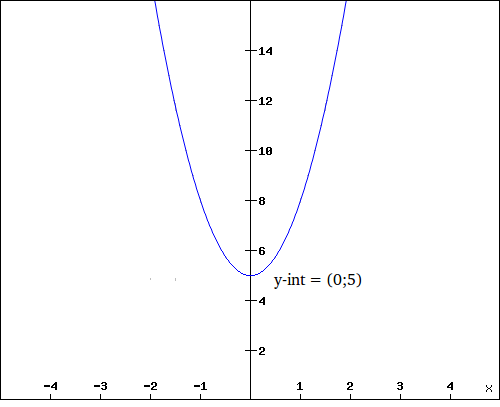
\includegraphics{[width=280px]col11306.imgs/m39345_parabola.png} % ;parabola.png;;;6.0;8.5;
\vspace{2pt}
\vspace{.1in}
\end{center}
\end{figure}       
\end{enumerate}
\end{exercise}
\end{mdframed}
}
\noindent
The following video shows one method of graphing parabolas. Note that in this video the term vertex is used in place of turning point. The vertex and the turning point are the same thing.
\setcounter{subfigure}{0}
\begin{figure}[H] % horizontal\label{m39345*parabola-1}
\textnormal{Khan academy video on graphing parabolas - 1}\vspace{.1in} \nopagebreak
\label{m39345*yt-media1}\label{m39345*yt-video1}
\raisebox{-5 pt}{ 
\includegraphics[width=0.5cm]{col11306.imgs/summary_www.png}} { (Video:  MG10019 )}
\vspace{2pt}
\vspace{.1in}
\end{figure}       \par 
\subsection*{Exercise:  parabolas }
\nopagebreak
\begin{enumerate}[noitemsep, label=\textbf{\arabic*}. ] 
\item Show that if $a<0$ that the range of $f(x)=a{x}^{2}+q$ is $\{f(x):f(x)\in (-\infty ;q]\}$.
\item Draw the graph of the function $y=-{x}^{2}+4$ showing all intercepts with the axes.
\item Two parabolas are drawn: $g:y=a{x}^{2}+p$ and $h:y=b{x}^{2}+q$.
\setcounter{subfigure}{0}
\begin{center}
\scalebox{1} % Change this value to rescale the drawing.
{
\begin{pspicture}(0,-2.61)(9.072187,2.61)
\psline[linewidth=0.04cm,arrowsize=0.05291667cm 2.0,arrowlength=1.4,arrowinset=0.4]{->}(0.0,-0.57)(9.04,-0.57 )
\psline[linewidth=0.04cm,arrowsize=0.05291667cm 2.0,arrowlength=1.4,arrowinset=0.4]{->}(4.54,-2.59)(4.56,2.59)
\psbezier[linewidth=0.04](1.8801522,2.249799)(2.0476475,1.0067352)(2.6697726,-0.42756912)(2.9090517 ,-0.81005025)(3.1483305,-1.1925315)(3.6508162,-1.83)(4.584004,-1.83)
\psbezier[linewidth=0.04](7.24,2.249799)(7.0725045,1.0067352)(6.4503794,-0.42756912)(6.2111006,-0.81005025)(5.971822,-1.1925315)(5.469336,-1.83)(4.536148 ,-1.83)
\psbezier[linewidth=0.04](1.2402416,-2.409998)(1.4477341,-1.215622)(2.2184203,0.16250414)(2.5148382,0.53000444)(2.811256,0.8975047)(3.4337332,1.5100052)(4.5897627,1.5100052)
\psbezier[linewidth=0.04](7.88,-2.409998 )(7.672508,-1.215622)(6.901821,0.16250414)(6.6054034,0.53000444)(6.3089857,0.8975047)(5.686508,1.5100052)(4.530479,1.5100052)
\usefont{T1}{ptm}{m}{it}
\rput(4.8129687,2.48){y}
\usefont{T1}{ptm}{m}{it}
\rput(8.908281 ,-0.3){x}
\usefont{T1}{ptm}{m}{n}
\rput(4.2504687,1.73){\footnotesize 23}
\usefont{T1}{ptm}{m}{n}
\rput(4.269219,-2.07){\footnotesize -9}
\usefont{T1}{ptm}{m}{n}
\rput(1.730625,0.39){\footnotesize (-4; 7)} 
\usefont{T1}{ptm}{m}{n}
\rput(7.240625,0.39){\footnotesize (4; 7)}
\usefont{T1}{ptm}{m}{n}
\rput(6.4275,-0.81){\footnotesize 3}
\usefont{T1}{ptm}{m}{it}
\rput(7.369219,1.87){\footnotesize g}
\usefont{T1}{ptm}{m}{it} 
\rput{-0.1}(0.0029207817,0.01384337){\rput(7.9021873,-1.69){\footnotesize h}}
\end{pspicture} 
}       
\end{center}
\begin{enumerate}[noitemsep, label=\textbf{\alph*}. ] 
\item Find the values of $a$ and $p$.
\item Find the values of $b$ and $q$.
\item Find the values of $x$ for which $a{x}^{2}+p\ge b{x}^{2}+q$.
\item For what values of $x$ is $g$ increasing ?
\end{enumerate}
  \end{enumerate}

\par \raisebox{-5 pt}{
\includegraphics[width=0.5cm]{col11306.imgs/summary_www.png}} Find the answers with the shortcodes:
\par \begin{tabular}[h]{cccccc}
(1.) lxD  &  (2.) lxW  &  (3.) lxZ  & \end{tabular}
%          \section{ Hyperbolic functions}
%     \nopagebreak
%             \label{m39341} $ \hspace{-5pt}\begin{array}{cccccccccccc}   
\includegraphics[width=0.75cm]{col11306.imgs/summary_fullmarks.png} &   \end{array} $ \hspace{2 pt}\raisebox{-5 pt}{} {(section shortcode: MG10020 )} \par 
%     
%     
%     

\section{Hyperbolic functions of the form $y=\frac{a}{x}+q$}
\nopagebreak
\subsection*{Plotting the graph}           
Functions of the form $y=\frac{a}{x}+q$ are known as hyperbolic functions. The general form of the graph of this function is shown in Figure~1.27.\par 
\setcounter{subfigure}{0}
\begin{figure}[tbp]
\begin{center}
\begin{pspicture}(-5,-2)(5,5)
%\psgrid
\psset{yunit=0.75,xunit=0.75}
\psaxes[arrows=<->](0,0)(-5,-2.667)(5,6)
\psplot[plotstyle=curve,arrows=<->]{-5}{-0.25}{x -1 exp 2 add}
\psplot[plotstyle=curve,arrows=<->]{0.25}{5}{x -1 exp 2 add}
\psplot[linestyle=dotted,plotstyle=curve]{-5}{2}{x 2 add}
\end{pspicture}
\caption{General shape and position of the graph of a function of the form $f(x)=\frac{a}{x} + q$.}
\label{fig:mf:g:hyperbola10}
\end{center}
\end{figure}      

\subsection*{ Investigating the effects of a and q }
\nopagebreak
\begin{enumerate}[noitemsep, label=\textbf{\arabic*}. ] 
\item On the same set of axes, plot the following graphs:
\begin{enumerate}[noitemsep, label=\textbf{\alph*}. ] 
\item $a(x)=\frac{-2}{x}+1$
\item $b(x)=\frac{-1}{x}+1$
\item $c(x)=\frac{0}{x}+1$
\item $d(x)=\frac{+1}{x}+1$
\item $e(x)=\frac{+2}{x}+1$\end{enumerate}
Use your results to deduce the effect of $a$.
\item On the same set of axes, plot the following graphs:
\begin{enumerate}[noitemsep, label=\textbf{\alph*}. ] 
\item $f(x)=\frac{1}{x}-2$
\item $g(x)=\frac{1}{x}-1$
\item $h(x)=\frac{1}{x}+0$\
item $j(x)=\frac{1}{x}+1$
\item $k(x)=\frac{1}{x}+2$\end{enumerate}
Use your results to deduce the effect of $q$.
\end{enumerate}
You should have found that the value of $a$ affects whether the graph is located in the first and third quadrants of Cartesian plane.\par 
You should have also found that the value of $q$ affects whether the graph lies above the $x$-axis ($q>0$) or below the $x$-axis ($q<0$).\par 
These different properties are summarised in Table 1.10. The axes of symmetry for each graph are shown as a dashed line.\par 
\begin{table}[htb]
\begin{center}
\caption{Table summarising general shapes and positions of functions of the form $y=\frac{a}{x} + q$. The axes of symmetry are shown as dashed lines.}
\label{tab:mf:graphs:summaryhyp10}
\begin{tabular}{|c|c|c|}\hline
& $a>0$&$a<0$\\\hline
$q>0$&
\begin{pspicture}(-1.2,-1.2)(1.2,1.2)
%\psgrid
\psset{xunit=0.2,yunit=0.2}
\psaxes[arrows=<->,dx=0,Dx=10,dy=0,Dy=10](0,0)(-5,-5)(5,5)
\psplot[plotstyle=curve,arrows=<->]{-5}{-0.25}{x -1 exp 2 add}
\psplot[plotstyle=curve,arrows=<->]{0.25}{5}{x -1 exp 2 add}
\psplot[linestyle=dotted,plotstyle=curve]{-4}{4}{x 2 add}
\end{pspicture}
&
\begin{pspicture}(-1.2,-1.2)(1.2,1.2)
%\psgrid
\psset{xunit=0.2,yunit=0.2}
\psaxes[arrows=<->,dx=0,Dx=10,dy=0,Dy=10](0,0)(-5,-5)(5,5)
\psplot[plotstyle=curve,arrows=<->]{-5}{-0.25}{x -1 exp neg 2 add}
\psplot[plotstyle=curve,arrows=<->]{0.25}{5}{x -1 exp neg 2 add}
\psplot[linestyle=dotted,plotstyle=curve]{-4}{4}{x neg 2 add}
\end{pspicture}
\\\hline
$q<0$&
\begin{pspicture}(-1.2,-1.2)(1.2,1.2)
%\psgrid
\psset{xunit=0.2,yunit=0.2}
\psaxes[arrows=<->,dx=0,Dx=10,dy=0,Dy=10](0,0)(-5,-5)(5,5)
\psplot[plotstyle=curve,arrows=<->]{-5}{-0.25}{x -1 exp 2 sub}
\psplot[plotstyle=curve,arrows=<->]{0.25}{5}{x -1 exp 2 sub}
\psplot[linestyle=dotted,plotstyle=curve]{-4}{4}{x 2 sub}
\end{pspicture}
&
\begin{pspicture}(-1.2,-1.2)(1.2,1.2)
%\psgrid
\psset{xunit=0.2,yunit=0.2}
\psaxes[arrows=<->,dx=0,Dx=10,dy=0,Dy=10](0,0)(-5,-5)(5,5)
\psplot[plotstyle=curve,arrows=<->]{-5}{-0.25}{x -1 exp neg 2 sub}
\psplot[plotstyle=curve,arrows=<->]{0.25}{5}{x -1 exp neg 2 sub}
\psplot[linestyle=dotted,plotstyle=curve]{-2}{4}{x neg 2 sub}
\end{pspicture}
\\\hline
\end{tabular}
\end{center}
\end{table}
\par
\subsection*{Discovering the characteristics}  
\subsection*{Domain and range}
\nopagebreak
For $y=\frac{a}{x}+q$, the function is undefined for $x=0$. The domain is therefore $\{x:x\in \mathbb{R},x\ne 0\}$.\par 
We see that $y=\frac{a}{x}+q$ can be re-written as:\par 
\nopagebreak\noindent{}
\begin{equation*}
\begin{array}{ccc}\hfill y& =& \frac{a}{x}+q\hfill \\ \hfill y-q& =& \frac{a}{x}\hfill \\ \hfill \mbox{If}\phantom{\rule{3pt}{0ex}}x\; \ne \;  0 \phantom{\rule{3pt}{0ex}}\mbox{then}:(y-q)x& =& a\hfill \\ \hfill x& =& \frac{a}{y-q}\hfill \end{array}
\end{equation*}
This shows that the function is undefined at $y=q$. Therefore the range of $f(x)=\frac{a}{x}+q$ is $\{f(x):f(x)\in (-\infty ;q)\cup (q;\infty )\}$.\par 
For example, the domain of $g(x)=\frac{2}{x}+2$ is $\{x:x\in \mathbb{R},x\ne 0\}$ because $g(x)$ is undefined at $x=0$.\par 
\nopagebreak\noindent{}
\begin{equation*}
\begin{array}{ccc}\hfill y& =& \frac{2}{x}+2\hfill \\ \hfill (y-2)& =& \frac{2}{x}\hfill \\ \hfill \mbox{If}\phantom{\rule{4pt}{0ex}}x\; \ne \;  0 \phantom{\rule{4pt}{0ex}}\mbox{then}:x(y-2)& =& 2\hfill \\ \hfill x& =& \frac{2}{y-2}\hfill \end{array}
\end{equation*}
We see that $g(x)$ is undefined at $y=2$. Therefore the range is $\{g(x):g(x)\in (-\infty ;2)\cup (2;\infty )\}$.\par 

\subsection*{Intercepts}
\nopagebreak
For functions of the form, $y=\frac{a}{x}+q$, the intercepts with the $x$ and $y$ axis is calculated by setting $x=0$ for the $y$-intercept and by setting $y=0$ for the $x$-intercept.\par 
The $y$-intercept is calculated as follows:\par 
\nopagebreak\noindent{}
\begin{equation*}
\begin{array}{ccc}\hfill y& =& \frac{a}{x}+q\hfill \\ \hfill {y}_{int}& =& \frac{a}{0}+q\hfill \end{array}
\end{equation*}
which is undefined because we are dividing by $0$. Therefore there is no $y$-intercept.\par 
For example, the $y$-intercept of $g(x)=\frac{2}{x}+2$ is given by setting $x=0$ to get:\par 
\nopagebreak\noindent{}
\begin{equation*}
\begin{array}{ccc}\hfill y& =& \frac{2}{x}+2\hfill \\ \hfill {y}_{int}& =& \frac{2}{0}+2\hfill \end{array}
\end{equation*}
which is undefined.\par 
The $x$-intercepts are calculated by setting $y=0$ as follows:\par 
\nopagebreak\noindent{}
\begin{equation*}
\begin{array}{ccc}\hfill y& =& \frac{a}{x}+q\hfill \\ \hfill 0& =& \frac{a}{{x}_{int}}+q\hfill \\ \hfill \frac{a}{{x}_{int}}& =& -q\hfill \\ \hfill a& =& -q({x}_{int})\hfill \\ \hfill {x}_{int}& =& \frac{a}{-q}\hfill \end{array}
\end{equation*}
For example, the $x$-intercept of $g(x)=\frac{2}{x}+2$ is given by setting $x=0$ to get:\par 
\nopagebreak\noindent{}
\begin{equation*}
\begin{array}{ccc}\hfill y& =& \frac{2}{x}+2\hfill \\ \hfill 0& =& \frac{2}{{x}_{int}}+2\hfill \\ \hfill -2& =& \frac{2}{{x}_{int}}\hfill \\ \hfill -2({x}_{int})& =& 2\hfill \\ \hfill {x}_{int}& =& \frac{2}{-2}\hfill \\ \hfill {x}_{int}& =& -1\hfill \end{array}
\end{equation*}

\subsection*{Asymptotes}
\nopagebreak
There are two asymptotes for functions of the form $y=\frac{a}{x}+q$. Just a reminder, an asymptote is a straight or curved line, which the graph of a function will approach, but never touch. They are determined by examining the domain and range.\par 
We saw that the function was undefined at $x=0$ and for $y=q$. Therefore the asymptotes are $x=0$ and $y=q$.\par 
For example, the domain of $g(x)=\frac{2}{x}+2$ is $\{x:x\in \mathbb{R},x\ne 0\}$ because $g(x)$ is undefined at $x=0$. We also see that $g(x)$ is undefined at $y=2$. Therefore the range is $\{g(x):g(x)\in (-\infty ;2)\cup (2;\infty )\}$.\par 
From this we deduce that the asymptotes are at $x=0$ and $y=2$.\par 

\subsection*{Sketching graphs of the form $f(x)=\frac{a}{x}+q$}
\nopagebreak
In order to sketch graphs of functions of the form, $f(x)=\frac{a}{x}+q$, we need to determine four characteristics:\par 
\begin{enumerate}[noitemsep, label=\textbf{\arabic*}. ] 
\item domain and range
\item asymptotes
\item $y$-intercept
\item $x$-intercept
\end{enumerate}
For example, sketch the graph of $g(x)=\frac{2}{x}+2$. Mark the intercepts and asymptotes.\par 
We have determined the domain to be $\{x:x\in \mathbb{R},x\ne 0\}$ and the range to be $\{g(x):g(x)\in (-\infty ;2)\cup (2;\infty )\}$. Therefore the asymptotes are at $x=0$ and $y=2$.\par 
There is no $y$-intercept and the $x$-intercept is ${x}_{int}=-1$.\par 
\setcounter{subfigure}{0}
\begin{figure}[tbp]
\begin{center}
\begin{pspicture}(-5,-3)(5,6)
%\psgrid
\psset{yunit=0.75,xunit=0.75}
\psaxes[arrows=<->](0,0)(-5,-4)(5,7)
\psplot[plotstyle=curve,arrows=<->]{-5}{-0.4}{x -1 exp 2 mul 2 add}
\psplot[plotstyle=curve,arrows=<->]{0.4}{5}{x -1 exp 2 mul 2 add}
\psline[linestyle=dashed](-5,2)(5,2)
\end{pspicture}
\caption{Graph of $g(x)=\frac{2}{x} + 2$.}
\label{fig:mf:g:hyperbolasketchexample}
\end{center}
\end{figure}       
\par
\label{m39341*eid75993}\vspace{.5cm} 
\noindent
\hspace*{-30pt}
\includegraphics[width=0.5in]{col11306.imgs/pspencil2.png}   \raisebox{25mm}{   
\begin{mdframed}[linewidth=4, leftmargin=40, rightmargin=40]  
\begin{exercise}
\noindent\textbf{Exercise 1.5: Drawing a hyperbola}
\label{m39341*probid734}\label{m39341*id6245}
Draw the graph of $y=\frac{-4}{x}+7$.\par 
\vspace{5pt}
\noindent\textbf{Solution to Exercise }
\begin{enumerate}[noitemsep, label=\textbf{Step} \textbf{\arabic*}. ] 
\leftskip=20pt\rightskip=\leftskip
\item The domain is: $\{x:x\in \mathbb{R},x\ne 0\}$ and the range is: $\{f(x):f(x)\in (-\infty ;7)\cup (7;\infty )\}$.
\item We look at the domain and range to determine where the asymptotes lie. From the domain we see that the function is undefined when $x=0$, so there is one asymptote at $x=0$. The other asymptote is found from the range. The function is undefined at $y=q$ and so the second asymptote is at $y=7$
\item There is no y-intercept for graphs of this form.\item The x-intercept occurs when $y=0$. Calculating the x-intercept gives:
\nopagebreak\noindent{}
\begin{equation*}
\begin{array}{ccc}\hfill y& =& \frac{-4}{x}+7\hfill \\ \hfill 0& =& \frac{-4}{x}+7\hfill \\ \hfill -7& =& \frac{-4}{x}\hfill \\ \hfill {x}_{\mathrm{int}}& =& \frac{4}{7}\hfill \end{array}
\end{equation*}
So there is one x-intercept at $(\frac{4}{7};0)$.\item Putting all this together gives us the following graph:
\setcounter{subfigure}{0}
\begin{figure}[H] % horizontal\label{m39341*uid12479}
\begin{center}
\label{m39341*uid12479!!!underscore!!!media}\label{m39341*uid12479!!!underscore!!!printimage}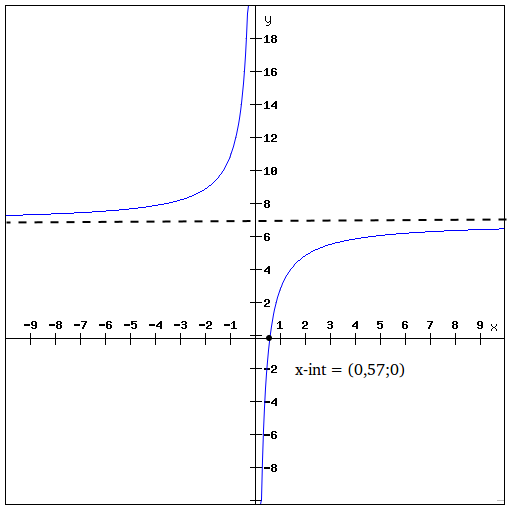
\includegraphics[width=280px]{col11306.imgs/m39341_hyperbola1.png} % ;hyperbola1.png;;;6.0;8.5;
\vspace{2pt}
\vspace{.1in}
\end{center}
\end{figure}       
\end{enumerate}
\end{exercise}
\end{mdframed}
}
\noindent

\subsection*{Exercises: Hyperbolic Graphs }
\nopagebreak
\begin{enumerate}[noitemsep, label=\textbf{\arabic*}. ] 
\item Using graph (grid) paper, draw the graph of $xy=-6$.
\begin{enumerate}[noitemsep, label=\textbf{\alph*}. ] 
\item Does the point $(-2; 3)$ lie on the graph ? Give a reason for your answer.
\item Why is the point $(-2; -3)$ not on the graph ?
\item If the $x$-value of a point on the drawn graph is $0,25$ what is the corresponding $y$-value ?
\item What happens to the $y$-values as the $x$-values become very large ?
\item With the line $y=-x$ as line of symmetry, what is the point symmetrical to $(-2; 3)$ ?
\end{enumerate}
  \item Draw the graph of $xy=8$.
\begin{enumerate}[noitemsep, label=\textbf{\alph*}. ] 
\item How would the graph $y=\frac{8}{3}+3$ compare with that of $xy=8$? Explain your answer fully.
\item Draw the graph of $y=\frac{8}{3}+3$ on the same set of axes.
\end{enumerate}
  \end{enumerate}

\par \raisebox{-5 pt}{
\includegraphics[width=0.5cm]{col11306.imgs/summary_www.png}} Find the answers with the shortcodes:
\par \begin{tabular}[h]{cccccc}
(1.) lxB  &  (2.) lxK  & \end{tabular}
% 
%          \section{ Exponential functions}
%     \nopagebreak
%             \label{m39348} $ \hspace{-5pt}\begin{array}{cccccccccccc}   
\includegraphics[width=0.75cm]{col11306.imgs/summary_fullmarks.png} &   \end{array} $ \hspace{2 pt}\raisebox{-5 pt}{} {(section shortcode: MG10021 )} \par 
%     
%     
%     
%     
%     
%     

\section{Exponential functions of the form $y=a{b}^{(x)}+q$}
\nopagebreak
\subsection*{Plotting the graph}         
Functions of the form $y=a{b}^{(x)}+q$ are known as exponential functions. The general shape of a graph of a function of this form is shown in Figure~1.34.\par 
\setcounter{subfigure}{0}
\begin{figure}[H]
\begin{center}
\begin{pspicture}(-5,-1)(5,4)
%\psgrid
\psset{yunit=0.75,xunit=0.75}
\psaxes[arrows=<->](0,0)(-5,-1)(5,5)
\psplot[plotstyle=curve,arrows=<->]{-5}{1.2}{2 x exp 2 add}
\end{pspicture}
\caption{General shape and position of the graph of a function of the form $f(x)=ab^{(x)} + q$.}
\label{fig:mf:g:exponential10}
\end{center}
\end{figure}     

\subsection*{ Investigating the effects of a and q}
\nopagebreak
\begin{enumerate}[noitemsep, label=\textbf{\arabic*}. ] 
\item On the same set of axes, plot the following graphs:
\begin{enumerate}[noitemsep, label=\textbf{\alph*}. ] 
\item $a(x)=-2\ensuremath{\cdot}{b}^{(x)}+1$
\item $b(x)=-1\ensuremath{\cdot}{b}^{(x)}+1$
\item $c(x)=0\ensuremath{\cdot}{b}^{(x)}+1$
\item $d(x)=1\ensuremath{\cdot}{b}^{(x)}+1$
\item $e(x)=2\ensuremath{\cdot}{b}^{(x)}+1$\end{enumerate}
Use your results to deduce the effect of $a$.
\item On the same set of axes, plot the following graphs:
\begin{enumerate}[noitemsep, label=\textbf{\alph*}. ] 
\item $f(x)=1\ensuremath{\cdot}{b}^{(x)}-2$
\item $g(x)=1\ensuremath{\cdot}{b}^{(x)}-1$
\item $h(x)=1\ensuremath{\cdot}{b}^{(x)}+0$
\item $j(x)=1\ensuremath{\cdot}{b}^{(x)}+1$
\item $k(x)=1\ensuremath{\cdot}{b}^{(x)}+2$\end{enumerate}
Use your results to deduce the effect of $q$.
\end{enumerate}
You should have found that the value of $a$ affects whether the graph curves upwards ($a>0$) or curves downwards ($a<0$).\par 
You should have also found that the value of $q$ affects the position of the $y$-intercept.\par 
These different properties are summarised in Table 1.11.\par 
\begin{table}[htb]
\begin{center}
\caption{Table summarising general shapes and positions of functions of the form $y=ab^{(x)} + q$.}
\label{tab:mf:graphs:summaryexp10}
\begin{tabular}{|c|c|c|}\hline
& $a>0$&$a<0$\\\hline
$q>0$&
\begin{pspicture}(-1.2,-1.2)(1.2,1.2)
\psset{xunit=0.2,yunit=0.2}
\psaxes[arrows=<->,dx=0,Dx=10,dy=0,Dy=10](0,0)(-5,-5)(5,5)
\psplot[plotstyle=curve,arrows=<->]{-5}{2}{2 x exp 2 add}
\end{pspicture}
&
\begin{pspicture}(-1.2,-1.2)(1.2,1.2)
%\psgrid
\psset{xunit=0.2,yunit=0.2}
\psaxes[arrows=<->,dx=0,Dx=10,dy=0,Dy=10](0,0)(-5,-5)(5,5)
\psplot[plotstyle=curve,arrows=<->]{-5}{2}{2 x exp -1 mul 2 add}
\end{pspicture}
\\\hline
$q<0$&
\begin{pspicture}(-1.2,-1.2)(1.2,1.2)
%\psgrid
\psset{xunit=0.2,yunit=0.2}
\psaxes[arrows=<->,dx=0,Dx=10,dy=0,Dy=10](0,0)(-5,-5)(5,5)
\psplot[plotstyle=curve,arrows=<->]{-5}{2}{2 x exp 2 sub}
\end{pspicture}
&
\begin{pspicture}(-1.2,-1.2)(1.2,1.2)
%\psgrid
\psset{xunit=0.2,yunit=0.2}
\psaxes[arrows=<->,dx=0,Dx=10,dy=0,Dy=10](0,0)(-5,-5)(5,5)
\psplot[plotstyle=curve,arrows=<->]{-5}{2}{2 x exp -1 mul 2 sub}
\end{pspicture}
\\\hline
\end{tabular}
\end{center}
\end{table}
\par
\subsection*{Discovering the characteristics}

\subsection*{Domain and range}
\nopagebreak
For $y=a{b}^{(x)}+q$, the function is defined for all real values of $x$. Therefore, the domain is $\{x:x\in \mathbb{R}\}$.\par 
The range of $y=a{b}^{(x)}+q$ is dependent on the sign of $a$.\par 
If $a>0$ then:\par 
\nopagebreak\noindent{}
\begin{equation*}
\begin{array}{ccc}\hfill {b}^{(x)}& \ge & 0\hfill \\ \hfill a\ensuremath{\cdot}{b}^{(x)}& \ge & 0\hfill \\ \hfill a\ensuremath{\cdot}{b}^{(x)}+q& \ge & q\hfill \\ \hfill f(x)& \ge & q\hfill \end{array}
\end{equation*}
Therefore, if $a>0$, then the range is $\{f(x):f(x)\in [q;\infty )\}$.\par 
If $a<0$ then:\par 
\nopagebreak\noindent{}
\begin{equation*}
\begin{array}{ccc}\hfill {b}^{(x)}& \le & 0\hfill \\ \hfill a\ensuremath{\cdot}{b}^{(x)}& \le & 0\hfill \\ \hfill a\ensuremath{\cdot}{b}^{(x)}+q& \le & q\hfill \\ \hfill f(x)& \le & q\hfill \end{array}
\end{equation*}
Therefore, if $a<0$, then the range is $\{f(x):f(x)\in (-\infty ;q]\}$.\par 
For example, the domain of $g(x)=3\ensuremath{\cdot}{2}^{x}+2$ is $\{x:x\in \mathbb{R}\}$.
For the range,\par 
\nopagebreak\noindent{}
\begin{equation*}
\begin{array}{ccc}\hfill {2}^{x}& \ge & 0\hfill \\ \hfill 3\ensuremath{\cdot}{2}^{x}& \ge & 0\hfill \\ \hfill 3\ensuremath{\cdot}{2}^{x}+2& \ge & 2\hfill \end{array}
\end{equation*}
Therefore the range is $\{g(x):g(x)\in [2;\infty )\}$.\par 

\subsection*{Intercepts}
\nopagebreak
For functions of the form, $y=a{b}^{(x)}+q$, the intercepts with the $x$ and $y$ axis is calculated by setting $x=0$ for the $y$-intercept and by setting $y=0$ for the $x$-intercept.\par 
The $y$-intercept is calculated as follows:\par 
\nopagebreak\noindent{}
\begin{equation*}
\begin{array}{ccc}\hfill y& =& a{b}^{(x)}+q\hfill \\ \hfill {y}_{int}& =& a{b}^{(0)}+q\hfill \\ & =& a(1)+q\hfill \\ & =& a+q\hfill \end{array}
\end{equation*}
For example, the $y$-intercept of $g(x)=3\ensuremath{\cdot}{2}^{x}+2$ is given by setting $x=0$ to get:\par 
\nopagebreak\noindent{}
\begin{equation*}
\begin{array}{ccc}\hfill y& =& 3\ensuremath{\cdot}{2}^{x}+2\hfill \\ \hfill {y}_{int}& =& 3\ensuremath{\cdot}{2}^{0}+2\hfill \\ & =& 3+2\hfill \\ & =& 5\hfill \end{array}
\end{equation*}
The $x$-intercepts are calculated by setting $y=0$ as follows:\par 
\nopagebreak\noindent{}
\begin{equation*}
\begin{array}{ccc}\hfill y& =& a{b}^{(x)}+q\hfill \\ \hfill 0& =& a{b}^{({x}_{int})}+q\hfill \\ \hfill a{b}^{({x}_{int})}& =& -q\hfill \\ \hfill {b}^{({x}_{int})}& =& -\frac{q}{a}\hfill \end{array}
\end{equation*}
Which only has a real solution if either $a<0$ or $q<0$. Otherwise, the graph of the function of form $y=a{b}^{(x)}+q$ does not have any $x$-intercepts.\par 
For example, the $x$-intercept of $g(x)=3\ensuremath{\cdot}{2}^{x}+2$ is given by setting $y=0$ to get:\par 
\nopagebreak\noindent{}
\begin{equation*}
\begin{array}{ccc}\hfill y& =& 3\ensuremath{\cdot}{2}^{x}+2\hfill \\ \hfill 0& =& 3\ensuremath{\cdot}{2}^{{x}_{int}}+2\hfill \\ \hfill -2& =& 3\ensuremath{\cdot}{2}^{{x}_{int}}\hfill \\ \hfill {2}^{{x}_{int}}& =& \frac{-2}{3}\hfill \end{array}
\end{equation*}
which has no real solution. Therefore, the graph of $g(x)=3\ensuremath{\cdot}{2}^{x}+2$ does not have any $x$-intercepts.\par 

\subsection*{Asymptotes}
\nopagebreak
Functions of the form $y=a{b}^{(x)}+q$ have a single horizontal asymptote. The asymptote can be determined by examining the range.\par 
We have seen that the range is controlled by the value of q. If $a>0$, then the range is $\{f(x):f(x)\in [q;\infty )\}$.And if $a>0$, then the range is $\{f(x):f(x)\in [q;\infty )\}$.\par 
This shows that the function tends towards the value of q as $x\to -\infty $. Therefore the horizontal asymptote lies at $x=q$.
\par 

\subsection*{Sketching graphs of the form $f(x)=a{b}^{(x)}+q$}
\nopagebreak
In order to sketch graphs of functions of the form, $f(x)=a{b}^{(x)}+q$, we need to determine four characteristics:\par 
\begin{enumerate}[noitemsep, label=\textbf{\arabic*}. ] 
\item domain and range
\item asymptote
\item $y$-intercept
\item $x$-intercept
\end{enumerate}
For example, sketch the graph of $g(x)=3\ensuremath{\cdot}{2}^{x}+2$. Mark the intercepts.\par 
We have determined the domain to be $\{x:x\in \mathbb{R}\}$ and the range to be $\{g(x):g(x)\in [2,\infty )\}$.\par 
The $y$-intercept is ${y}_{int}=5$ and there are no $x$-intercepts.\par 
\setcounter{subfigure}{0}
\begin{figure}[htbp]
\begin{center}
\begin{pspicture}(-5,-1)(5,6)
%\psgrid
\psset{yunit=0.75,xunit=0.75}
\psaxes[arrows=<->](0,0)(-5,-1)(5,7)
\psplot[plotstyle=curve,arrows=<->]{-5}{0.5}{2 x exp 3 mul 2 add}
\end{pspicture}
\caption{Graph of $g(x)=3\cdot 2^{x} + 2$.}
\label{fig:mf:g:exponentialsketchexample10}
\end{center}
\end{figure}      


\par
\label{m39348*eid78823}\vspace{.5cm} 
\noindent
\hspace*{-30pt}
\includegraphics[width=0.5in]{col11306.imgs/pspencil2.png}   \raisebox{25mm}{   
\begin{mdframed}[linewidth=4, leftmargin=40, rightmargin=40]  
\begin{exercise}
\noindent\textbf{Exercise 1.6: Drawing an exponential graph}

Draw the graph of $y=-2.{3}^{x}+5$.\par 
\vspace{5pt}
\noindent\textbf{Solution to Exercise }
\begin{enumerate}[noitemsep, label=\textbf{Step} \textbf{\arabic*}. ] 
\leftskip=20pt\rightskip=\leftskip\item The domain is: $\{x:x\in \mathbb{R}\}$ and the range is: $\{f(x):f(x)\in (-\infty ;5]\}$.
\item There is one asymptote for functions of this form. This occurs at $y=q$. So the asymptote for this graph is at $y=5$
\item The y-intercept occurs when $x=0$.
\nopagebreak\noindent{}
\begin{equation*}
\begin{array}{ccc}\hfill y& =& -2.{3}^{x}+5\hfill \\ \hfill y& =& -2.{3}^{0}+5\hfill \\ \hfill y& =& -2(1)+5\hfill \\ \hfill {y}_{\mathrm{int}}& =& 7\hfill \end{array}
\end{equation*}
So there is one y-intercept at $(0,7)$.
\item The x-intercept occurs when $y=0$. Calculating the x-intercept gives:
\nopagebreak\noindent{}
\begin{equation*}
\begin{array}{ccc}\hfill y& =& -2.{3}^{x}+5\hfill \\ \hfill 0& =& -2.{3}^{x}+5\hfill \\ \hfill -5& =& -2.{3}^{x}\hfill \\ \hfill {3}^{{x}_{\mathrm{int}}}& =& \frac{5}{2}\hfill \\ \hfill {x}_{\mathrm{int}}& =& 0,83\hfill \end{array}
\end{equation*}
So there is one x-intercept at $(0,83,0)$.\item Putting all this together gives us the following graph:
\setcounter{subfigure}{0}
\begin{figure}[H] % horizontal\label{m39348*uid12329}
\begin{center}
\label{m39348*uid12329!!!underscore!!!media}\label{m39348*uid123279!!!underscore!!!printimage}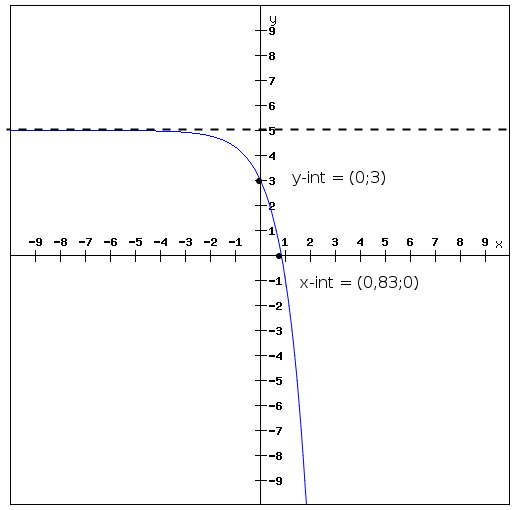
\includegraphics[width=300px]{col11306.imgs/m39348_exponent1.png} % ;exponent1.png;;;6.0;8.5;
\vspace{2pt}
\vspace{.1in}
\end{center}
\end{figure}       
\end{enumerate}
\end{exercise}
\end{mdframed}
}
\noindent

\subsection*{ Exercise: Exponential Functions and Graphs }
\nopagebreak
\begin{enumerate}[noitemsep, label=\textbf{\arabic*}. ] 
\item Draw the graphs of $y={2}^{x}$ and $y={(\frac{1}{2})}^{x}$ on the same set of axes.
\begin{enumerate}[noitemsep, label=\textbf{\alph*}. ] 
\item Is the $x$-axis and asymptote or and axis of symmetry to both graphs ? Explain your answer.
\item Which graph is represented by the equation $y={2}^{-x}$ ? Explain your answer.
\item Solve the equation ${2}^{x}={(\frac{1}{2})}^{x}$ graphically and check that your answer is correct by using substitution.
\item Predict how the graph $y=2.{2}^{x}$ will compare to $y={2}^{x}$ and then draw the graph of $y=2.{2}^{x}$ on the same set of axes.
\end{enumerate}
  \item The curve of the exponential function $f$ in the accompanying diagram cuts the y-axis at the point $A(0; 1)$ and $B(2; 4)$ is on $f$.
\setcounter{subfigure}{0}
\begin{center}
\scalebox{1} % Change this value to rescale the drawing.
{
\begin{pspicture}(0,-3.19)(6.3184376,3.21)
\psdots[dotsize=0.12](5.0,1.49)
\psdots[dotsize= 0.12](1.0,-1.51)
\psbezier[linewidth=0.04](0.0,-1.81)(5.0,-0.41)(5.5,2.59)(5.6,3.19)
\rput(5.7725,1.7){B(2,4)}
\rput(1.7076563,-1.8){A(0,1)}
\rput(1.0,-2.51){\psaxes[linewidth=0.04,arrowsize=0.05291667cm 2.0,arrowlength= 1.4,arrowinset=0.4,ticksize=0.08cm,dx=2.0cm,dy=1.0cm]{<->}(0,0)(-1,0)(5,5)}
\rput(5.994375,-2.8){x}
\rput(0.564375,2.5){f}
\end{pspicture} 
}     
\end{center}
\begin{enumerate}[noitemsep, label=\textbf{\alph*}. ] 
\item Determine the equation of the function $f$.
\item Determine the equation of $h$, the function of which the curve is the reflection of the curve of $f$ in the $x$-axis.
\item Determine the range of $h$.
\end{enumerate}
  \end{enumerate}

\par \raisebox{-5 pt}{
\includegraphics[width=0.5cm]{col11306.imgs/summary_www.png}} Find the answers with the shortcodes:
\par \begin{tabular}[h]{cccccc}
(1.) lxk  &  (2.) lx0  & \end{tabular}

\section{Trigonometric functions}
\nopagebreak
This section describes the graphs of trigonometric functions.\par 

\subsection{Graph of $y=sin~\theta $}
\subsection*{Plotting the graph}
\nopagebreak
Complete the following table, using your calculator to calculate the values. Then plot the values with $sin\theta $ on the $y$-axis and $\theta $ on the $x$-axis. Round answers to $1$ decimal place.\par 
% \textbf{m39414*id83562}\par
% how many colspecs?  8
% name: cnx:colspec
% colnum: 1
% colwidth: 10*
% latex-name: columna
% colname: c1
% align/tgroup-align/default: //left
% -------------------------
% name: cnx:colspec
% colnum: 2
% colwidth: 10*
% latex-name: columnb
% colname: c2
% align/tgroup-align/default: //left
% -------------------------
% name: cnx:colspec
% colnum: 3
% colwidth: 10*
% latex-name: columnc
% colname: c3
% align/tgroup-align/default: //left
% -------------------------
% name: cnx:colspec
% colnum: 4
% colwidth: 10*
% latex-name: columnd
% colname: c4
% align/tgroup-align/default: //left
% -------------------------
% name: cnx:colspec
% colnum: 5
% colwidth: 10*
% latex-name: columne
% colname: c5
% align/tgroup-align/default: //left
% -------------------------
% name: cnx:colspec
% colnum: 6
% colwidth: 10*
% latex-name: columnf
% colname: c6
% align/tgroup-align/default: //left
% -------------------------
% name: cnx:colspecPlotting the g
% colnum: 7
% colwidth: 10*
% latex-name: columng
% colname: c7
% align/tgroup-align/default: //left
% -------------------------
% name: cnx:colspec
% colnum: 8
% colwidth: 10*
% latex-name: columnh
% colname: c8
% align/tgroup-align/default: //left
% -------------------------
\setlength\mytablespace{16\tabcolsep}
\addtolength\mytablespace{9\arrayrulewidth}
\setlength\mytablewidth{\linewidth}
\setlength\mytableroom{\mytablewidth}
\addtolength\mytableroom{-\mytablespace}
\setlength\myfixedwidth{0pt}
\setlength\mystarwidth{\mytableroom}
\addtolength\mystarwidth{-\myfixedwidth}
\divide\mystarwidth 80
% ----- Table with code
% \begin{table}[H]
% \\ '' '0'
\begin{center}
\label{m39414*id83562}
\noindent
\tabletail{%
\hline
\multicolumn{8}{|p{\mytableroom}|}{\raggedleft \small \sl continued on next page}\\
\hline
}
\tablelasttail{}
\begin{xtabular*}{\mytablewidth}[t]{|p{10\mystarwidth}|p{10\mystarwidth}|p{10\mystarwidth}|p{10\mystarwidth}|p{10\mystarwidth}|p{10\mystarwidth}|p{10\mystarwidth}|p{10\mystarwidth}|}\hline
% count in rowspan-info-nodeset: 8
% align/colidx: left,1
% rowcount: '0' | start: 'false' | colidx: '1'
% Formatting a regular cell and recurring on the next sibling
    $\theta $
    &
% align/colidx: left,2
% rowcount: '0' | start: 'false' | colidx: '2'
% Formatting a regular cell and recurring on the next sibling
0${}^{\circ }$ &
% align/colidx: left,3
% rowcount: '0' | start: 'false' | colidx: '3'
% Formatting a regular cell and recurring on the next sibling
30${}^{\circ }$ &Plotting the g
% align/colidx: left,4
% rowcount: '0' | start: 'false' | colidx: '4'
% Formatting a regular cell and recurring on the next sibling
60${}^{\circ }$ &
% align/colidx: left,5
% rowcount: '0' | start: 'false' | colidx: '5'
% Formatting a regular cell and recurring on the next sibling
90${}^{\circ }$ &
% align/colidx: left,6
% rowcount: '0' | start: 'false' | colidx: '6'
% Formatting a regular cell and recurring on the next sibling
120${}^{\circ }$ &
% align/colidx: left,7
% rowcount: '0' | start: 'false' | colidx: '7'
% Formatting a regular cell and recurring on the next sibling
150${}^{\circ }$ &
% align/colidx: left,8
% rowcount: '0' | start: 'false' | colidx: '8'
% Formatting a regular cell and recurring on the next sibling
% make-rowspan-placeholders
% rowspan info: col1 '0' | 'false' | '' || col2 '0' | 'false' | '' || col3 '0' | 'false' | '' || col4 '0' | 'false' | '' || col5 '0' | 'false' | '' || col6 '0' | 'false' | '' || col7 '0' | 'false' | '' || col8 '0' | 'false' | ''
\tabularnewline\cline{1-1}\cline{2-2}\cline{3-3}\cline{4-4}\cline{5-5}\cline{6-6}\cline{7-7}\cline{8-8}
%--------------------------------------------------------------------
% align/colidx: left,1
% rowcount: '0' | start: 'false' | colidx: '1'
% Formatting a regular cell and recurring on the next sibling
    $sin\theta $
    &
% align/colidx: left,2
% rowcount: '0' | start: 'false' | colidx: '2'
% Formatting a regular cell and recurring on the next sibling
&
% align/colidx: left,3
% rowcount: '0' | start: 'false' | colidx: '3'
% Formatting a regular cell and recurring on the next sibling
&
% align/colidx: left,4
% rowcount: '0' | start: 'false' | colidx: '4'
% Formatting a regular cell and recurring on the next sibling
&
% align/colidx: left,5
% rowcount: '0' | start: 'false' | colidx: '5'
% Formatting a regular cell and recurring on the next sibling
&
% align/colidx: left,6
% rowcount: '0' | start: 'false' | colidx: '6'sub
% Formatting a regular cell and recurring on the next sibling
&
% align/colidx: left,7
% rowcount: '0' | start: 'false' | colidx: '7'
% Formatting a regular cell and recurring on the next sibling
&
% align/colidx: left,8
% rowcount: '0' | start: 'false' | colidx: '8'
% Formatting a regular cell and recurring on the next sibling
% make-rowspan-placeholders
% rowspan info: col1 '0' | 'false' | '' || col2 '0' | 'false' | '' || col3 '0' | 'false' | '' || col4 '0' | 'false' | '' || col5 '0' | 'false' | '' || col6 '0' | 'false' | '' || col7 '0' | 'false' | '' || col8 '0' | 'false' | ''
\tabularnewline\cline{1-1}\cline{2-2}\cline{3-3}\cline{4-4}\cline{5-5}\cline{6-6}\cline{7-7}\cline{8-8}
%--------------------------------------------------------------------
% align/colidx: left,1
% rowcount: '0' | start: 'false' | colidx: '1'
% Formatting a regular cell and recurring on the next sibling
    $\theta $
    &
% align/colidx: left,2
% rowcount: '0' | start: 'false' | colidx: '2'
% Formatting a regular cell and recurring on the next sibling
180${}^{\circ }$ &
% align/colidx: left,3
% rowcount: '0' | start: 'false' | colidx: '3'
% Formatting a regular cell and recurring on the next sibling
210${}^{\circ }$ &
% align/colidx: left,4
% rowcount: '0' | start: 'false' | colidx: '4'
% Formatting a regular cell and recurring on the next sibling
240${}^{\circ }$ &
% align/colidx: left,5
% rowcount: '0' | start: 'false' | colidx: '5'
% Formatting a regular cell and recurring on the next sibling
270${}^{\circ }$ &
% align/colidx: left,6
% rowcount: '0' | start: 'false' | colidx: '6'
% Formatting a regular cell and recurring on the next sibling
300${}^{\circ }$ &
% align/colidx: left,7
% rowcount: '0' | start: 'false' | colidx: '7'
% Formatting a regular cell and recurring on the next sibling
330${}^{\circ }$ &
% align/colidx: left,8
% rowcount: '0' | start: 'false' | colidx: '8'
% Formatting a regular cell and recurring on the next sibling
360${}^{\circ }$% make-rowspan-placeholders
% rowspan info: col1 '0' | 'false' | '' || col2 '0' | 'false' | '' || col3 '0' | 'false' | '' || col4 '0' | 'false' | '' || col5 '0' | 'false' | '' || col6 '0' | 'false' | '' || col7 '0' | 'false' | '' || col8 '0' | 'false' | ''
\tabularnewline\cline{1-1}\cline{2-2}\cline{3-3}\cline{4-4}\cline{5-5}\cline{6-6}\cline{7-7}\cline{8-8}
%--------------------------------------------------------------------
% align/colidx: left,1
% rowcount: '0' | start: 'false' | colidx: '1'
% Formatting a regular cell and recurring on the next sibling
    $sin\theta $
    &
% align/colidx: left,2
% rowcount: '0' | start: 'false' | colidx: '2'
% Formatting a regular cell and recurring on the next sibling
&
% align/colidx: left,3
% rowcount: '0' | start: 'false' | colidx: '3'
% Formatting a regular cell and recurring on the next sibling
&
% align/colidx: left,4
% rowcount: '0' | start: 'false' | colidx: '4'
% Formatting a regular cell and recurring on the next sibling
&
% align/colidx: left,5
% rowcount: '0' | start: 'false' | colidx: '5'
% Formatting a regular cell and recurring on the next sibling
&
% align/colidx: left,6Plotting 
% rowcount: '0' | start: 'false' | colidx: '6'
% Formatting a regular cell and recurring on the next sibling
&
% align/colidx: left,7
% rowcount: '0' | start: 'false' | colidx: '7'
% Formatting a regular cell and recurring on the next sibling
&
% align/colidx: left,8
% rowcount: '0' | start: 'false' | colidx: '8'
% Formatting a regular cell and recurring on the next sibling
% make-rowspan-placeholders
% rowspan info: col1 '0' | 'false' | '' || col2 '0' | 'false' | '' || col3 '0' | 'false' | '' || col4 '0' | 'false' | '' || col5 '0' | 'false' | '' || col6 '0' | 'false' | '' || col7 '0' | 'false' | '' || col8 '0' | 'false' | ''
\tabularnewline\cline{1-1}\cline{2-2}\cline{3-3}\cline{4-4}\cline{5-5}\cline{6-6}\cline{7-7}\cline{8-8}
%--------------------------------------------------------------------
% My position: 0
% my spanname: 
% my ct of spanspec: 0
% my column-count: 8
% align/colidx: center,1
\multicolumn{8}{|p{\dimexpr10\mystarwidth+10\mystarwidth+10\mystarwidth+10\mystarwidth+10\mystarwidth+10\mystarwidth+10\mystarwidth+10\mystarwidth+14\tabcolsep+7\arrayrulewidth\relax}|}{}
% rowspan info: col1 '0' | 'false' | '' || col2 '0' | 'false' | '' || col3 '0' | 'false' | '' || col4 '0' | 'false' | '' || col5 '0' | 'false' | '' || col6 '0' | 'false' | '' || col7 '0' | 'false' | '' || col8 '0' | 'false' | ''
\tabularnewline\cline{1-1}\cline{2-2}\cline{3-3}\cline{4-4}\cline{5-5}\cline{6-6}\cline{7-7}\cline{8-8}
%--------------------------------------------------------------------
% My position: 0
% my spanname: 
% my ct of spanspec: 0
% my column-count: 8
% align/colidx: center,1
\multicolumn{8}{|p{\dimexpr10\mystarwidth+10\mystarwidth+10\mystarwidth+10\mystarwidth+10\mystarwidth+10\mystarwidth+10\mystarwidth+10\mystarwidth+14\tabcolsep+7\arrayrulewidth\relax}|}{
\setcounter{subfigure}{0}
\label{m39414*id84030}
\begin{center}
\begin{pspicture}(0,-1)(4,1)
\psset{xunit=2}
%\psgrid[gridcolor=gray]
\psset{xunit=0.01111}
\psaxes[dx=30,Dx=30]{<->}(0,0)(0,-1.2)(370,1.2)
\end{pspicture}
\end{center}    
  }
% rowspan info: col1 '0' | 'false' | '' || col2 '0' | 'false' | '' || col3 '0' | 'false' | '' || col4 '0' | 'false' | '' || col5 '0' | 'false' | '' || col6 '0' | 'false' | '' || col7 '0' | 'false' | '' || col8 '0' | 'false' | ''
\tabularnewline\cline{1-1}\cline{2-2}\cline{3-3}\cline{4-4}\cline{5-5}\cline{6-6}\cline{7-7}\cline{8-8}
%--------------------------------------------------------------------
\end{xtabular*}
\end{center}
\begin{center}{\small\bfseries Table 14.4}\end{center}
%\end{table}
\par
\label{m39414*id84056}Let us look back at our values for $sin\theta $\par 
\begin{table}[H]
% \begin{table}[H]
% \\ '' '0'
\begin{center}
\label{m39414*id84073}
\noindent
\tabletail{%
\hline
\multicolumn{7}{|p{\mytableboxwidth}|}{\raggedleft \small \sl continued on next page}\\
\hline
}
\tablelasttail{}
\begin{xtabular}[t]{|l|l|l|l|l|l|l|}\hline
    $\theta $
    &
    ${0}^{\circ }$
    &
    ${30}^{\circ }$
    &
    ${45}^{\circ }$Plotting 
    &
    ${60}^{\circ }$
    &
    ${90}^{\circ }$
    &
    ${180}^{\circ }$
  % make-rowspan-placeholders
\tabularnewline\cline{1-1}\cline{2-2}\cline{3-3}\cline{4-4}\cline{5-5}\cline{6-6}\cline{7-7}
%--------------------------------------------------------------------
    $sin\theta $
    &
0 &
    $\frac{1}{2}$
    &
    $\frac{1}{\sqrt{2}}$
    &
    $\frac{\sqrt{3}}{2}$
    &
1 &
0% make-rowspan-placeholders
\tabularnewline\cline{1-1}\cline{2-2}\cline{3-3}\cline{4-4}\cline{5-5}\cline{6-6}\cline{7-7}
%--------------------------------------------------------------------
\end{xtabular}
\end{center}Plotting 
\begin{center}{\small\bfseries Table 14.5}\end{center}
\begin{caption}{\small\bfseries Table 14.5}\end{caption}
\end{table}
\par
As you can see, the function $sin\theta $ has a value of $0$ at $\theta ={0}^{\circ }$. Its value then smoothly increases until $\theta ={90}^{\circ }$ when its value is $1$. We also know that it later decreases to $0$ when $\theta ={180}^{\circ }$. Putting all this together we can start to picture the full extent of the sine graph. The sine graph is shown in Figure~14.23. Notice the wave shape, with each wave having a length of ${360}^{\circ }$. We say the graph has a period of ${360}^{\circ }$. The height of the wave above (or below) the $x$-axis is called the wave's amplitude. Thus the maximum amplitude of the sine-wave is $1$, and its minimum amplitude is $-1$.\par 
\setcounter{subfigure}{0}
\begin{figure}[h]
\begin{center}
\begin{pspicture}(-6,-2)(6,2)
\psaxes[Ox=0, Dx=180, dx=2]{<->}(0,0)(-4.5,-1.5)(4.5,1.5)
\psplot[xunit=0.0111,yunit=1.0, plotpoints=1000]{-360}{360}{x sin}
\rput(5.1,-.3){Degrees}
\psline[linestyle=dashed](0, 1)(4, 1)
\psline[linestyle=dashed](0, -1)(4, -1)
\end{pspicture}
\caption{The graph of $\sin \theta$.}
\label{trig:sin}
\end{center}
\end{figure}
      

\subsection*{Graphs of the form $y=asin(x)+q$}
\nopagebreak
In the equation, $y=asin(x)+q$, $a$ and $q$ are constants and have different effects on the graph of the function. The general shape of the graph of functions of this form is shown in Figure~14.24 for the function $f(\theta )=2sin\theta +3$.\par 
\setcounter{subfigure}{0}
\begin{figure}[!ht]
\begin{center}
\begin{pspicture}(-4,-2)(4,6)
%\psgrid[gridcolor=gray]
\psset{yunit=1,xunit=0.01111}
\psaxes[dx=90,Dx=90]{<->}(0,0)(-360,-2)(360,6)
\psplot[plotstyle=curve,arrows=<->]{-360}{360}{x sin 2 mul 3 add}
\rput(5.1,-.3){Degrees}
\end{pspicture}
\caption{Graph of $f(\theta)=2 \sin \theta +3$}
\label{fig:mt:g:sin}
\end{center}
\end{figure}   

\subsection*{Investigating the effects of a and q}
\nopagebreak
\begin{enumerate}[noitemsep, label=\textbf{\arabic*}. ] 
\item On the same set of axes, plot the following graphs:
\begin{enumerate}[noitemsep, label=\textbf{\alph*}. ] 
\item $a(\theta )=sin\theta -2$
\item $b(\theta )=sin\theta -1$
\item $c(\theta )=sin\theta $
\item $d(\theta )=sin\theta +1$
\item $e(\theta )=sin\theta +2$
\end{enumerate}
Use your results to deduce the effect of $q$.
\item On the same set of axes, plot the following graphs:
\begin{enumerate}[noitemsep, label=\textbf{\alph*}. ] 
\item $f(\theta )=-2\ensuremath{\cdot}sin\theta $
\item $g(\theta )=-1\ensuremath{\cdot}sin\theta $
\item $h(\theta )=0\ensuremath{\cdot}sin\theta $
\item $j(\theta )=1\ensuremath{\cdot}sin\theta $
\item $k(\theta )=2\ensuremath{\cdot}sin\theta $\end{enumerate}
Use your results to deduce the effect of $a$.
\end{enumerate}
You should have found that the value of $a$ affects the height of the peaks of the graph. As the magnitude of $a$ increases, the peaks get higher. As it decreases, the peaks get lower.\par 
$q$ is called the vertical shift. If $q=2$, then the whole sine graph shifts up $2$ units. If $q=-1$, the whole sine graph shifts down $1$ unit.\par 
These different properties are summarised in Table 14.6.\par 
\begin{table}[htb]
\begin{center}
\caption{Table summarising general shapes and positions of graphs of functions of the form $y=a \sin(x) + q$.}
\label{tab:mt:g:summarysin10}
\begin{tabular}{|c||c|c|}\hline
& $a>0$&$a<0$\\\hline\hline
$q>0$&
\begin{pspicture}(-1.2,-0.6)(1.2,1.2)
\psset{yunit=0.5,xunit=0.0111}
\psaxes[arrows=<->,dx=0,Dx=720,dy=0,Dy=10,xunit=0.25](0,0)(-450,-1)(450,2)
\psplot[plotstyle=curve,arrows=<->,xunit=0.25]{-360}{360}{x sin 0.5 add}
\rput(5.1,-.3){Degrees}
\end{pspicture}
&
\begin{pspicture}(-1.2,-0.6)(1.2,1.2)
\psset{yunit=0.5,xunit=0.0111}
\psaxes[arrows=<->,dx=0,Dx=720,dy=0,Dy=10,xunit=0.25](0,0)(-450,-1)(450,2)
\psplot[plotstyle=curve,arrows=<->,xunit=0.25]{-360}{360}{x sin neg 0.5 add}
\rput(5.1,-.3){Degrees}
\end{pspicture}\\\hline
$q<0$&
\begin{pspicture}(-1.2,-1.2)(1.2,0.6)
%\psgrid
\psset{yunit=0.5,xunit=0.0111}
\psaxes[arrows=<->,dx=0,Dx=720,dy=0,Dy=10,xunit=0.25](0,0)(-450,-2)(450,1)
\psplot[plotstyle=curve,arrows=<->,xunit=0.25]{-360}{360}{x sin 0.5 sub}
\rput(5.1,-.3){Degrees}
\end{pspicture}
&
\begin{pspicture}(-1.2,-1.2)(1.2,0.6)
%\psgrid
\psset{yunit=0.5,xunit=0.0111}
\psaxes[arrows=<->,dx=0,Dx=720,dy=0,Dy=10,xunit=0.25](0,0)(-450,-2)(450,1)
\psplot[plotstyle=curve,arrows=<->,xunit=0.25]{-360}{360}{x sin neg 0.5 sub}
\rput(5.1,-.3){Degrees}
\end{pspicture}\\\hline
\end{tabular}
\end{center}
\end{table}
\par

\subsection*{Discovering the characteristics}
\subsection*{Domain and range}
\nopagebreak
For $f(\theta )=asin(\theta )+q$, the domain is $\{\theta :\theta \in \mathbb{R}\}$ because there is no value of $\theta \in \mathbb{R}$ for which $f(\theta )$ is undefined.\par 
The range of $f(\theta )=asin\theta +q$ depends on whether the value for $a$ is positive or negative. We will consider these two cases separately.\par 
If $a>0$ we have:\par 
\nopagebreak\noindent{}
\begin{equation*}
\begin{array}{ccc}\hfill -1\le sin\theta & \le & 1\hfill \\ \hfill -a\le asin\theta & \le & a\hfill \\ \hfill -a+q\le asin\theta +q& \le & a+q\hfill \\ \hfill -a+q\le f(\theta )& \le & a+q\hfill \end{array}
\end{equation*}
This tells us that for all values of $\theta $, $f(\theta )$ is always between $-a+q$ and $a+q$. Therefore if $a>0$, the range of $f(\theta )=asin\theta +q$ is $\{f(\theta ):f(\theta )\in [-a+q,a+q]\}$.\par 
Similarly, it can be shown that if $a<0$, the range of $f(\theta )=asin\theta +q$ is $\{f(\theta ):f(\theta )\in [a+q,-a+q]\}$. This is left as an exercise.\par 

\begin{tabular}{cc}
\hspace*{-50pt}\raisebox{-8 mm}{ 
\includegraphics[width=0.5in]{col11306.imgs/pstip2.png}  }& 
\begin{minipage}{0.85\textwidth}
\begin{note}
{tip: }The easiest way to find the range is simply to look for the "bottom" and the "top" of the graph.
\end{note}
\end{minipage}
\end{tabular}
\par

\subsection*{Intercepts}
\nopagebreak
The $y$-intercept, ${y}_{int}$, of $f(\theta )=asin(x)+q$ is simply the value of $f(\theta )$ at $\theta ={0}^{\circ }$.\par 
\nopagebreak\noindent{}
\begin{equation*}
\begin{array}{ccc}\hfill {y}_{int}& =& f({0}^{\circ })\hfill \\ & =& asin({0}^{\circ })+q\hfill \\ & =& a(0)+q\hfill \\ & =& q\hfill \end{array}
\end{equation*}



\subsection{Graph of $y=cos~\theta $}
\subsection*{Plotting the graph}
\nopagebreak
 Complete the following table, using your calculator to calculate the values correct to $1$ decimal place. Then plot the values with $cos\theta $ on the $y$-axis and $\theta $ on the $x$-axis.\par 
% \textbf{m39414*id86399}\par
% how many colspecs?  8
% name: cnx:colspec
% colnum: 1
% colwidth: 10*
% latex-name: columna
% colname: c1
% align/tgroup-align/default: //left
% -------------------------
% name: cnx:colspec
% colnum: 2
% colwidth: 10*
% latex-name: columnb
% colname: c2
% align/tgroup-align/default: //left
% -------------------------
% name: cnx:colspec
% colnum: 3
% colwidth: 10*
% latex-name: columnc
% colname: c3
% align/tgroup-align/default: //left
% -------------------------
% name: cnx:colspec
% colnum: 4
% colwidth: 10*
% latex-name: columnd
% colname: c4
% align/tgroup-align/default: //left
% -------------------------
% name: cnx:colspec
% colnum: 5
% colwidth: 10*
% latex-name: columne
% colname: c5
% align/tgroup-align/default: //left
% -------------------------
% name: cnx:colspec
% colnum: 6
% colwidth: 10*
% latex-name: columnf
% colname: c6
% align/tgroup-align/default: //left
% -------------------------
% name: cnx:colspec
% colnum: 7
% colwidth: 10*
% latex-name: columng
% colname: c7
% align/tgroup-align/default: //left
% -------------------------
% name: cnx:colspec
% colnum: 8
% colwidth: 10*
% latex-name: columnh
% colname: c8
% align/tgroup-align/default: //left
% -------------------------
\setlength\mytablespace{16\tabcolsep}
\addtolength\mytablespace{9\arrayrulewidth}
\setlength\mytablewidth{\linewidth}
\setlength\mytableroom{\mytablewidth}
\addtolength\mytableroom{-\mytablespace}
\setlength\myfixedwidth{0pt}
\setlength\mystarwidth{\mytableroom}
\addtolength\mystarwidth{-\myfixedwidth}
\divide\mystarwidth 80subsub
% ----- Table with code
% \begin{table}[H]
% \\ '' '0'
\begin{center}
\label{m39414*id86399}
\noindent
\tabletail{%
\hline
\multicolumn{8}{|p{\mytableroom}|}{\raggedleft \small \sl continued on next page}\\
\hline
}
\tablelasttail{}
\begin{xtabular*}{\mytablewidth}[t]{|p{10\mystarwidth}|p{10\mystarwidth}|p{10\mystarwidth}|p{10\mystarwidth}|p{10\mystarwidth}|p{10\mystarwidth}|p{10\mystarwidth}|p{10\mystarwidth}|}\hline
% count in rowspan-info-nodeset: 8
% align/colidx: left,1
% rowcount: '0' | start: 'false' | colidx: '1'
% Formatting a regular cell and recurring on the next sibling
    $\theta $
    &
% align/colidx: left,2
% rowcount: '0' | start: 'false' | colidx: '2'
% Formatting a regular cell and recurring on the next sibling
0${}^{\circ }$ &
% align/colidx: left,3
% rowcount: '0' | start: 'false' | colidx: '3'
% Formatting a regular cell and recurring on the next sibling
30${}^{\circ }$ &
% align/colidx: left,4
% rowcount: '0' | start: 'false' | colidx: '4'
% Formatting a regular cell and recurring on the next sibling
60${}^{\circ }$ &
% align/colidx: left,5
% rowcount: '0' | start: 'false' | colidx: '5'
% Formatting a regular cell and recurring on the next sibling
90${}^{\circ }$ &
% align/colidx: left,6
% rowcount: '0' | start: 'false' | colidx: '6'
% Formatting a regular cell and recurring on the next sibling
120${}^{\circ }$ &
% align/colidx: left,7
% rowcount: '0' | start: 'false' | colidx: '7'
% Formatting a regular cell and recurring on the next sibling
150${}^{\circ }$ &
% align/colidx: left,8
% rowcount: '0' | start: 'false' | colidx: '8'
% Formatting a regular cell and recurring on the next sibling
% make-rowspan-placeholders
% rowspan info: col1 '0' | 'false' | '' || col2 '0' | 'false' | '' || col3 '0' | 'false' | '' || col4 '0' | 'false' | '' || col5 '0' | 'false' | '' || col6 '0' | 'false' | '' || col7 '0' | 'false' | '' || col8 '0' | 'false' | ''
\tabularnewline\cline{1-1}\cline{2-2}\cline{3-3}\cline{4-4}\cline{5-5}\cline{6-6}\cline{7-7}\cline{8-8}
%--------------------------------------------------------------------
% align/colidx: left,1
% rowcount: '0' | start: 'false' | colidx: '1'
% Formatting a regular cell and recurring on the next sibling
    $cos\theta $
    &
% align/colidx: left,2
% rowcount: '0' | start: 'false' | colidx: '2'
% Formatting a regular cell and recurring on the next sibling
&
% align/colidx: left,3
% rowcount: '0' | start: 'false' | colidx: '3'
% Formatting a regular cell and recurring on the next sibling
&
% align/colidx: left,4
% rowcount: '0' | start: 'false' | colidx: '4'
% Formatting a regular cell and recurring on the next sibling
&
% align/colidx: left,5
% rowcount: '0' | start: 'false' | colidx: '5'
% Formatting a regular cell and recurring on the next sibling
&
% align/colidx: left,6
% rowcount: '0' | start: 'false' | colidx: '6'
% Formatting a regular cell and recurring on the next sibling
&
% align/colidx: left,7
% rowcount: '0' | start: 'false' | colidx: '7'
% Formatting a regular cell and recurring on the next sibling
&
% align/colidx: left,8
% rowcount: '0' | start: 'false' | colidx: '8'
% Formatting a regular cell and recurring on the next sibling
% make-rowspan-placeholders
% rowspan info: col1 '0' | 'false' | '' || col2 '0' | 'false' | '' || col3 '0' | 'false' | '' || col4 '0' | 'false' | '' || col5 '0' | 'false' | '' || col6 '0' | 'false' | '' || col7 '0' | 'false' | '' || col8 '0' | 'false' | ''
\tabularnewline\cline{1-1}\cline{2-2}\cline{3-3}\cline{4-4}\cline{5-5}\cline{6-6}\cline{7-7}\cline{8-8}
%--------------------------------------------------------------------
% align/colidx: left,1
% rowcount: '0' | start: 'false' | colidx: '1'
% Formatting a regular cell and recurring on the next sibling
    $\theta $
    &
% align/colidx: left,2
% rowcount: '0' | start: 'false' | colidx: '2'
% Formatting a regular cell and recurring on the next sibling
180${}^{\circ }$ &
% align/colidx: left,3
% rowcount: '0' | start: 'false' | colidx: '3'
% Formatting a regular cell and recurring on the next sibling
210${}^{\circ }$ &
% align/colidx: left,4
% rowcount: '0' | start: 'false' | colidx: '4'
% Formatting a regular cell and recurring on the next sibling
240${}^{\circ }$ &
% align/colidx: left,5
% rowcount: '0' | start: 'false' | colidx: '5'
% Formatting a regular cell and recurring on the next sibling
270${}^{\circ }$ &
% align/colidx: left,6
% rowcount: '0' | start: 'false' | colidx: '6'
% Formatting a regular cell and recurring on the next sibling
300${}^{\circ }$ &
% align/colidx: left,7
% rowcount: '0' | start: 'false' | colidx: '7'
% Formatting a regular cell and recurring on the next sibling
330${}^{\circ }$ &
% align/colidx: left,8
% rowcount: '0' | start: 'false' | colidx: '8'
% Formatting a regular cell and recurring on the next sibling
360${}^{\circ }$% make-rowspan-placeholders
% rowspan info: col1 '0' | 'false' | '' || col2 '0' | 'false' | '' || col3 '0' | 'false' | '' || col4 '0' | 'false' | '' || col5 '0' | 'false' | '' || col6 '0' | 'false' | '' || col7 '0' | 'false' | '' || col8 '0' | 'false' | ''
\tabularnewline\cline{1-1}\cline{2-2}\cline{3-3}\cline{4-4}\cline{5-5}\cline{6-6}\cline{7-7}\cline{8-8}
%--------------------------------------------------------------------
% align/colidx: left,1
% rowcount: '0' | start: 'false' | colidx: '1'
% Formatting a regular cell and recurring on the next sibling
    $cos\theta $
    &
% align/colidx: left,2
% rowcount: '0' | start: 'false' | colidx: '2'
% Formatting a regular cell and recurring on the next sibling
&Functions
% align/colidx: left,3
% rowcount: '0' | start: 'false' | colidx: '3'
% Formatting a regular cell and recurring on the next sibling
&subsub
% align/colidx: left,4
% rowcount: '0' | start: 'false' | colidx: '4'
% Formatting a regular cell and recurring on the next sibling
&
% align/colidx: left,5
% rowcount: '0' | start: 'false' | colidx: '5'
% Formatting a regular cell and recurring on the next sibling
&
% align/colidx: left,6
% rowcount: '0' | start: 'false' | colidx: '6'
% Formatting a regular cell and recurring on the next sibling
&
% align/colidx: left,7
% rowcount: '0' | start: 'false' | colidx: '7'
% Formatting a regular cell and recurring on the next sibling
&
% align/colidx: left,8
% rowcount: '0' | start: 'false' | colidx: '8'
% Formatting a regular cell and recurring on the next sibling
% make-rowspan-placeholders
% rowspan info: col1 '0' | 'false' | '' || col2 '0' | 'false' | '' || col3 '0' | 'false' | '' || col4 '0' | 'false' | '' || col5 '0' | 'false' | '' || col6 '0' | 'false' | '' || col7 '0' | 'false' | '' || col8 '0' | 'false' | ''
\tabularnewline\cline{1-1}\cline{2-2}\cline{3-3}\cline{4-4}\cline{5-5}\cline{6-6}\cline{7-7}\cline{8-8}
%--------------------------------------------------------------------
% My position: 0
% my spanname: 
% my ct of spanspec: 0
% my column-count: 8
% align/colidx: center,1
\multicolumn{8}{|p{\dimexpr10\mystarwidth+10\mystarwidth+10\mystarwidth+10\mystarwidth+10\mystarwidth+10\mystarwidth+10\mystarwidth+10\mystarwidth+14\tabcolsep+7\arrayrulewidth\relax}|}{}
% rowspan info: col1 '0' | 'false' | '' || col2 '0' | 'false' | '' || col3 '0' | 'false' | '' || col4 '0' | 'false' | '' || col5 '0' | 'false' | '' || col6 '0' | 'false' | '' || col7 '0' | 'false' | '' || col8 '0' | 'false' | ''
\tabularnewline\cline{1-1}\cline{2-2}\cline{3-3}\cline{4-4}\cline{5-5}\cline{6-6}\cline{7-7}\cline{8-8}
%--------------------------------------------------------------------
% My position: 0
% my spanname: 
% my ct of spanspec: 0
% my column-count: 8
% align/colidx: center,1
\multicolumn{8}{|p{\dimexpr10\mystarwidth+10\mystarwidth+10\mystarwidth+10\mystarwidth+10\mystarwidth+10\mystarwidth+10\mystarwidth+10\mystarwidth+14\tabcolsep+7\arrayrulewidth\relax}|}{
\setcounter{subfigure}{0}
\begin{pspicture}(0,-1)(4,1)
\psset{xunit=2}
%\psgrid[gridcolor=gray]
\psset{xunit=0.01111}
\psaxes[dx=30,Dx=30]{<->}(0,0)(0,-1.2)(370,1.2)
\end{pspicture} 
  }
% rowspan info: col1 '0' | 'false' | '' || col2 '0' | 'false' | '' || col3 '0' | 'false' | '' || col4 '0' | 'false' | '' || col5 '0' | 'false' | '' || col6 '0' | 'false' | '' || col7 '0' | 'false' | '' || col8 '0' | 'false' | ''
\tabularnewline\cline{1-1}\cline{2-2}\cline{3-3}\cline{4-4}\cline{5-5}\cline{6-6}\cline{7-7}\cline{8-8}
%--------------------------------------------------------------------
\end{xtabular*}
\end{center}
\begin{center}{\small\bfseries Table 14.7}\end{center}
%\end{table}
\par
\label{m39414*id86892}Let us look back at our values for $cos\theta $\par 
% \textbf{m39414*uid46}\par
\begin{table}[H]
% \begin{table}[H]
% \\ '' '0'
\begin{center}
\label{m39414*id86909}
\noindent
\tabletail{%
\hline
\multicolumn{7}{|p{\mytableboxwidth}|}{\raggedleft \small \sl continued on next page}\\
\hline
}
\tablelasttail{}
\begin{xtabular}[t]{|l|l|l|l|l|l|l|}\hline
    $\theta $
    &
    ${0}^{\circ }$
    &
    ${30}^{\circ }$
    &
    ${45}^{\circ }$
    &
    ${60}^{\circ }$
    &
    ${90}^{\circ }$
    &
    ${180}^{\circ }$
  % make-rowspan-placeholders
\tabularnewline\cline{1-1}\cline{2-2}\cline{3-3}\cline{4-4}\cline{5-5}\cline{6-6}\cline{7-7}
%--------------------------------------------------------------------
    $cos\theta $
    &
1 &
    $\frac{\sqrt{3}}{2}$
    &
    $\frac{1}{\sqrt{2}}$
    &
    $\frac{1}{2}$
    &
0 &
    $-1$
  % make-rowspan-placeholders
\tabularnewline\cline{1-1}\cline{2-2}\cline{3-3}\cline{4-4}\cline{5-5}\cline{6-6}\cline{7-7}
%--------------------------------------------------------------------
\end{xtabular}
\end{center}
\begin{center}{\small\bfseries Table 14.8}\end{center}
\begin{caption}{\small\bfseries Table 14.8}\end{caption}
\end{table}
\par
If you look carefully, you will notice that the cosine of an angle $\theta $ is the same as the sine of the angle ${90}^{\circ }-\theta $. Take for example,\par 
\nopagebreak\noindent{}
\begin{equation*}
cos{60}^{\circ }=\frac{1}{2}=sin{30}^{\circ }=sin({90}^{\circ }-{60}^{\circ })
\end{equation*}
This tells us that in order to create the cosine graph, all we need to do is to shift the sine graph ${90}^{\circ }$ to the left. The graph of $cos\theta $ is shown in Figure~14.30. As the cosine graph is simply a shifted sine graph, it will have the same period and amplitude as the sine graph.\par 
\setcounter{subfigure}{0}
\begin{figure}[h]
\begin{center}
\begin{pspicture}(-6,-2)(6,2)
\psaxes[Ox=0, Dx=180, dx=2]{<->}(0,0)(-4.5,-1.5)(4.5,1.5)
%\psline[]{<-}(0,1.2)(1,1.2)
\psplot[xunit=0.0111,yunit=1.0, plotpoints=1000]{-360}{360}{x cos}
\rput(5.1,-.3){Degrees}
\end{pspicture}
\caption{The graph of $\cos \theta$.}
\label{trig:cos}
\end{center}
\end{figure}      

\subsection*{Graphs of the form $y=acos(x)+q$}
\nopagebreak
In the equation, $y=acos(x)+q$, $a$ and $q$ are constants and have different effects on the graph of the function. The general shape of the graph of functions of this form is shown in Figure~14.31 for the function $f(\theta )=2cos\theta +3$.\par 
\setcounter{subfigure}{0}
\begin{figure}[!ht]
\begin{center}
\begin{pspicture}(-4,-2)(4,6)
%\psgrid[gridcolor=gray]
\psset{yunit=1,xunit=0.01111}
\psaxes[dx=90,Dx=90]{<->}(0,0)(-360,-2)(360,6)
\psplot[plotstyle=curve,arrows=<->]{-360}{360}{x cos 2 mul 3 add}
\rput(5.1,-.3){Degrees}
\end{pspicture}
\caption{Graph of $f(\theta)=2 \cos \theta +3$}
\label{fig:mt:g:cos}
\end{center}
\end{figure}      

\subsection*{Investigating the effects of a and q}
\nopagebreak
\begin{enumerate}[noitemsep, label=\textbf{\arabic*}. ] 
\item On the same set of axes, plot the following graphs:
\begin{enumerate}[noitemsep, label=\textbf{\alph*}. ] 
\item $a(\theta )=cos\theta -2$
\item $b(\theta )=cos\theta -1$
\item $c(\theta )=cos\theta $
\item $d(\theta )=cos\theta +1$
\item $e(\theta )=cos\theta +2$\end{enumerate}
Use your results to deduce the effect of $q$.
\item On the same set of axes, plot the following graphs:
\begin{enumerate}[noitemsep, label=\textbf{\alph*}. ] 
\item $f(\theta )=-2\ensuremath{\cdot}cos\theta $
\item $g(\theta )=-1\ensuremath{\cdot}cos\theta $
\item $h(\theta )=0\ensuremath{\cdot}cos\theta $
\item $j(\theta )=1\ensuremath{\cdot}cos\theta $
\item $k(\theta )=2\ensuremath{\cdot}cos\theta $\end{enumerate}
Use your results to deduce the effect of $a$.
\end{enumerate}
You should have found that the value of $a$ affects the amplitude of the cosine graph in the same way it did for the sine graph.\par 
You should have also found that the value of $q$ shifts the cosine graph in the same way as it did the sine graph.\par 
These different properties are summarised in Table 14.9.\par 
\begin{table}[htb]
\begin{center}
\caption{Table summarising general shapes and positions of graphs of functions of the form $y=a \cos(x) + q$.}
\label{tab:mt:g:summarycos10}
\begin{tabular}{|c||c|c|}\hline
& $a>0$&$a<0$\\\hline\hline
$q>0$&
\begin{pspicture}(-1.2,-0.6)(1.2,1.2)
\psset{yunit=0.5,xunit=0.0111}
\psaxes[arrows=<->,dx=0,Dx=720,dy=0,Dy=10,xunit=0.25](0,0)(-450,-1)(450,2)
\psplot[plotstyle=curve,arrows=<->,xunit=0.25]{-360}{360}{x cos 0.5 add}
\end{pspicture}
&
\begin{pspicture}(-1.2,-0.6)(1.2,1.2)
\psset{yunit=0.5,xunit=0.0111}
\psaxes[arrows=<->,dx=0,Dx=720,dy=0,Dy=10,xunit=0.25](0,0)(-450,-1)(450,2)
\psplot[plotstyle=curve,arrows=<->,xunit=0.25]{-360}{360}{x cos neg 0.5 add}
\end{pspicture}\\\hline
$q<0$&
\begin{pspicture}(-1.2,-1.2)(1.2,0.6)
%\psgrid
\psset{yunit=0.5,xunit=0.0111}
\psaxes[arrows=<->,dx=0,Dx=720,dy=0,Dy=10,xunit=0.25](0,0)(-450,-2)(450,1)
\psplot[plotstyle=curve,arrows=<->,xunit=0.25]{-360}{360}{x cos 0.5 sub}
\end{pspicture}
&
\begin{pspicture}(-1.2,-1.2)(1.2,0.6)
%\psgrid
\psset{yunit=0.5,xunit=0.0111}
\psaxes[arrows=<->,dx=0,Dx=720,dy=0,Dy=10,xunit=0.25](0,0)(-450,-2)(450,1)
\psplot[plotstyle=curve,arrows=<->,xunit=0.25]{-360}{360}{x cos neg 0.5 sub}
\end{pspicture}\\\hline
\end{tabular}
\end{center}
\end{table}
\par

\subsection*{Discovering the characteristics}
\subsection*{Domain and range}
\nopagebreak
For $f(\theta )=acos(\theta )+q$, the domain is $\{\theta :\theta \in \mathbb{R}\}$ because there is no value of $\theta \in \mathbb{R}$ for which $f(\theta )$ is undefined.\par 
It is easy to see that the range of $f(\theta )$ will be the same as the range of $asin(\theta )+q$. This is because the maximum and minimum values of $acos(\theta )+q$ will be the same as the maximum and minimum values of $asin(\theta )+q$.\par 

\subsection*{Intercepts}
\nopagebreak
The $y$-intercept of $f(\theta )=acos(x)+q$ is calculated in the same way as for sine.\par 
\nopagebreak\noindent{}
\begin{equation*}
\begin{array}{ccc}\hfill {y}_{int}& =& f({0}^{\circ })\hfill \\ & =& acos({0}^{\circ })+q\hfill \\ & =& a(1)+q\hfill \\ & =& a+q\hfill \end{array}
\end{equation*}

\subsection*{Comparison of graphs of $y=sin~\theta $ and $y=cos~\theta $}
\nopagebreak
\setcounter{subfigure}{0}
\begin{figure}[h]
\begin{center}
\begin{pspicture}(-6,-2)(6,2)
\psaxes[Ox=0, Dx=180, dx=2]{<->}(0,0)(-4.5,-1.5)(4.5,1.5)
\psline[]{<-}(0,1.2)(1,1.2)
\psplot[xunit=0.0111, , yunit=1.0, plotpoints=1000, linestyle=dashed]{-360}{360}{x sin}
\psplot[xunit=0.0111,yunit=1.0, plotpoints=1000]{-360}{360}{x cos}
\rput(5.1,-.3){Degrees}
\rput(1.8,1.2){$90^\circ$ shift}
\end{pspicture}
\caption{The graph of $\cos \theta$ (solid-line) and the graph of $\sin \theta$ (dashed-line).}
\end{center}
\end{figure}    
Notice that the two graphs look very similar. Both oscillate up and down around the $x$-axis as you move along the axis. The distances between the peaks of the two graphs is the same and is constant along each graph. The height of the peaks and the depths of the troughs are the same.\par 
The only difference is that the $sin$ graph is shifted a little to the right of the $cos$ graph by 90${}^{\circ }$. That means that if you shift the whole $cos$ graph to the right by 90 ${}^{\circ }$ it will overlap perfectly with the $sin$ graph. You could also move the $sin$ graph by 90 ${}^{\circ }$to the left and it would overlap perfectly with the $cos$ graph. This means that:\par 
\nopagebreak\noindent{}
\begin{equation*}
\begin{array}{ccc}\hfill sin\theta & =& cos(\theta -90)(\mbox{shift the}\phantom{\rule{2.pt}{0ex}}cos\phantom{\rule{2.pt}{0ex}}\mbox{graph to the right})\hfill \\ & \mathbf{a}\mbox{nd}& \\ \hfill cos\theta & =& sin(\theta +90)(\mbox{shift the}\phantom{\rule{2.pt}{0ex}}sin\phantom{\rule{2.pt}{0ex}}\mbox{graph to the left})\hfill \end{array}
\end{equation*}

\subsection{Graph of $y=tan\theta $ }
\subsection*{Plotting the graph}
\nopagebreak
Complete the following table, using your calculator to calculate the values correct to 1 decimal place. Then plot the values with $tan\theta $ on the $y$-axis and $\theta $ on the $x$-axis.\par 
% \textbf{m39414*id89083}\par
% how many colspecs?  8
% name: cnx:colspec
% colnum: 1
% colwidth: 10*
% latex-name: columna
% colname: c1
% align/tgroup-align/default: //left
% -------------------------
% name: cnx:colspec
% colnum: 2
% colwidth: 10*
% latex-name: columnb
% colname: c2
% align/tgroup-align/default: //left
% -------------------------
% name: cnx:colspec
% colnum: 3
% colwidth: 10*
% latex-name: columnc
% colname: c3
% align/tgroup-align/default: //left
% -------------------------
% name: cnx:colspec
% colnum: 4
% colwidth: 10*
% latex-name: columnd
% colname: c4
% align/tgroup-align/default: //left
% -------------------------
% name: cnx:colspec
% colnum: 5
% colwidth: 10*
% latex-name: columne
% colname: c5
% align/tgroup-align/default: //left
% -------------------------
% name: cnx:colspec
% colnum: 6
% colwidth: 10*
% latex-name: columnf
% colname: c6
% align/tgroup-align/default: //left
% -------------------------
% name: cnx:colspec
% colnum: 7
% colwidth: 10*
% latex-name: columng
% colname: c7
% align/tgroup-align/default: //left
% -------------------------
% name: cnx:colspec
% colnum: 8
% colwidth: 10*
% latex-name: columnh
% colname: c8
% align/tgroup-align/default: //left
% -------------------------
\setlength\mytablespace{16\tabcolsep}
\addtolength\mytablespace{9\arrayrulewidth}
\setlength\mytablewidth{\linewidth}
\setlength\mytableroom{\mytablewidth}
\addtolength\mytableroom{-\mytablespace}
\setlength\myfixedwidth{0pt}
\setlength\mystarwidth{\mytableroom}
\addtolength\mystarwidth{-\myfixedwidth}
\divide\mystarwidth 80
% ----- Table with code
% \begin{table}[H]
% \\ '' '0'
\begin{center}
\label{m39414*id89083}
\noindent
\tabletail{%
\hline
\multicolumn{8}{|p{\mytableroom}|}{\raggedleft \small \sl continued on next page}\\
\hline
}
\tablelasttail{}
\begin{xtabular*}{\mytablewidth}[t]{|p{10\mystarwidth}|p{10\mystarwidth}|p{10\mystarwidth}|p{10\mystarwidth}|p{10\mystarwidth}|p{10\mystarwidth}|p{10\mystarwidth}|p{10\mystarwidth}|}\hline
% count in rowspan-info-nodeset: 8
% align/colidx: left,1
% rowcount: '0' | start: 'false' | colidx: '1'
% Formatting a regular cell and recurring on the next sibling
    $\theta $
    &
% align/colidx: left,2
% rowcount: '0' | start: 'false' | colidx: '2'
% Formatting a regular cell and recurring on the next sibling
0${}^{\circ }$ &
% align/colidx: left,3
% rowcount: '0' | start: 'false' | colidx: '3'
% Formatting a regular cell and recurring on the next sibling
30${}^{\circ }$ &
% align/colidx: left,4
% rowcount: '0' | start: 'false' | colidx: '4'
% Formatting a regular cell and recurring on the next sibling
60${}^{\circ }$ &
% align/colidx: left,5
% rowcount: '0' | start: 'false' | colidx: '5'
% Formatting a regular cell and recurring on the next sibling
90${}^{\circ }$ &
% align/colidx: left,6
% rowcount: '0' | start: 'false' | colidx: '6'
% Formatting a regular cell and recurring on the next sibling
120${}^{\circ }$ &
% align/colidx: left,7
% rowcount: '0' | start: 'false' | colidx: '7'
% Formatting a regular cell and recurring on the next sibling
150${}^{\circ }$ &
% align/colidx: left,8
% rowcount: '0' | start: 'false' | colidx: '8'
% Formatting a regular cell and recurring on the next sibling
% make-rowspan-placeholders
% rowspan info: col1 '0' | 'false' | '' || col2 '0' | 'false' | '' || col3 '0' | 'false' | '' || col4 '0' | 'false' | '' || col5 '0' | 'false' | '' || col6 '0' | 'false' | '' || col7 '0' | 'false' | '' || col8 '0' | 'false' | ''
\tabularnewline\cline{1-1}\cline{2-2}\cline{3-3}\cline{4-4}\cline{5-5}\cline{6-6}\cline{7-7}\cline{8-8}
%--------------------------------------------------------------------
% align/colidx: left,1
% rowcount: '0' | start: 'false' | colidx: '1'
% Formatting a regular cell and recurring on the next sibling
    $tan\theta $
    &
% align/colidx: left,2
% rowcount: '0' | start: 'false' | colidx: '2'
% Formatting a regular cell and recurring on the next sibling
&
% align/colidx: left,3
% rowcount: '0' | start: 'false' | colidx: '3'
% Formatting a regular cell and recurring on the next sibling
&
% align/colidx: left,4
% rowcount: '0' | start: 'false' | colidx: '4'
% Formatting a regular cell and recurring on the next sibling
&
% align/colidx: left,5
% rowcount: '0' | start: 'false' | colidx: '5'
% Formatting a regular cell and recurring on the next sibling
&
% align/colidx: left,6
% rowcount: '0' | start: 'false' | colidx: '6'
% Formatting a regular cell and recurring on the next sibling
&
% align/colidx: left,7
% rowcount: '0' | start: 'false' | colidx: '7'
% Formatting a regular cell and recurring on the next sibling
&
% align/colidx: left,8
% rowcount: '0' | start: 'false' | colidx: '8'
% Formatting a regular cell and recurring on the next sibling
% make-rowspan-placeholders
% rowspan info: col1 '0' | 'false' | '' || col2 '0' | 'false' | '' || col3 '0' | 'false' | '' || col4 '0' | 'false' | '' || col5 '0' | 'false' | '' || col6 '0' | 'false' | '' || col7 '0' | 'false' | '' || col8 '0' | 'false' | ''
\tabularnewline\cline{1-1}\cline{2-2}\cline{3-3}\cline{4-4}\cline{5-5}\cline{6-6}\cline{7-7}\cline{8-8}
%--------------------------------------------------------------------
% align/colidx: left,1
% rowcount: '0' | start: 'false' | colidx: '1'
% Formatting a regular cell and recurring on the next sibling
    $\theta $
    &
% align/colidx: left,2
% rowcount: '0' | start: 'false' | colidx: '2'
% Formatting a regular cell and recurring on the next sibling
180${}^{\circ }$ &
% align/colidx: left,3
% rowcount: '0' | start: 'false' | colidx: '3'
% Formatting a regular cell and recurring on the next sibling
210${}^{\circ }$ &
% align/colidx: left,4
% rowcount: '0' | start: 'false' | colidx: '4'
% Formatting a regular cell and recurring on the next sibling
240${}^{\circ }$ &
% align/colidx: left,5
% rowcount: '0' | start: 'false' | colidx: '5'
% Formatting a regular cell and recurring on the next sibling
270${}^{\circ }$ &
% align/colidx: left,6
% rowcount: '0' | start: 'false' | colidx: '6'
% Formatting a regular cell and recurring on the next sibling
300${}^{\circ }$ &
% align/colidx: left,7
% rowcount: '0' | start: 'false' | colidx: '7'
% Formatting a regular cell and recurring on the next sibling
330${}^{\circ }$ &
% align/colidx: left,8
% rowcount: '0' | start: 'false' | colidx: '8'
% Formatting a regular cell and recurring on the next sibling
360${}^{\circ }$% make-rowspan-placeholders
% rowspan info: col1 '0' | 'false' | '' || col2 '0' | 'false' | '' || col3 '0' | 'false' | '' || col4 '0' | 'false' | '' || col5 '0' | 'false' | '' || col6 '0' | 'false' | '' || col7 '0' | 'false' | '' || col8 '0' | 'false' | ''
\tabularnewline\cline{1-1}\cline{2-2}\cline{3-3}\cline{4-4}\cline{5-5}\cline{6-6}\cline{7-7}\cline{8-8}
%--------------------------------------------------------------------
% align/colidx: left,1
% rowcount: '0' | start: 'false' | colidx: '1'
% Formatting a regular cell and recurring on the next sibling
    $tan\theta $
    &
% align/colidx: left,2
% rowcount: '0' | start: 'false' | colidx: '2'
% Formatting a regular cell and recurring on the next sibling
&
% align/colidx: left,3
% rowcount: '0' | start: 'false' | colidx: '3'
% Formatting a regular cell and recurring on the next sibling
&
% align/colidx: left,4
% rowcount: '0' | start: 'false' | colidx: '4'
% Formatting a regular cell and recurring on the next sibling
&
% align/colidx: left,5
% rowcount: '0' | start: 'false' | colidx: '5'
% Formatting a regular cell and recurring on the next sibling
&
% align/colidx: left,6
% rowcount: '0' | start: 'false' | colidx: '6'
% Formatting a regular cell and recurring on the next sibling
&
% align/colidx: left,7
% rowcount: '0' | start: 'false' | colidx: '7'
% Formatting a regular cell and recurring on the next sibling
&
% align/colidx: left,8
% rowcount: '0' | start: 'false' | colidx: '8'
% Formatting a regular cell and recurring on the next sibling
% make-rowspan-placeholders
% rowspan info: col1 '0' | 'false' | '' || col2 '0' | 'false' | '' || col3 '0' | 'false' | '' || col4 '0' | 'false' | '' || col5 '0' | 'false' | '' || col6 '0' | 'false' | '' || col7 '0' | 'false' | '' || col8 '0' | 'false' | ''
\tabularnewline\cline{1-1}\cline{2-2}\cline{3-3}\cline{4-4}\cline{5-5}\cline{6-6}\cline{7-7}\cline{8-8}
%--------------------------------------------------------------------
% My position: 0
% my spanname: 
% my ct of spanspec: 0
% my column-count: 8
% align/colidx: center,1
\multicolumn{8}{|p{\dimexpr10\mystarwidth+10\mystarwidth+10\mystarwidth+10\mystarwidth+10\mystarwidth+10\mystarwidth+10\mystarwidth+10\mystarwidth+14\tabcolsep+7\arrayrulewidth\relax}|}{}
% rowspan info: col1 '0' | 'false' | '' || col2 '0' | 'false' | '' || col3 '0' | 'false' | '' || col4 '0' | 'false' | '' || col5 '0' | 'false' | '' || col6 '0' | 'false' | '' || col7 '0' | 'false' | '' || col8 '0' | 'false' | ''
\tabularnewline\cline{1-1}\cline{2-2}\cline{3-3}\cline{4-4}\cline{5-5}\cline{6-6}\cline{7-7}\cline{8-8}
%--------------------------------------------------------------------
% My position: 0
% my spanname: 
% my ct of spanspec: 0
% my column-count: 8
% align/colidx: center,1
\multicolumn{8}{|p{\dimexpr10\mystarwidth+10\mystarwidth+10\mystarwidth+10\mystarwidth+10\mystarwidth+10\mystarwidth+10\mystarwidth+10\mystarwidth+14\tabcolsep+7\arrayrulewidth\relax}|}{
\setcounter{subfigure}{0}
\begin{pspicture}(0,-1)(4,1)
\psset{xunit=2}
%\psgrid[gridcolor=gray]
\psset{xunit=0.01111}
\psaxes[dx=30,Dx=30]{<->}(0,0)(0,-1.2)(370,1.2)
\end{pspicture}   
  }
% rowspan info: col1 '0' | 'false' | '' || col2 '0' | 'false' | '' || col3 '0' | 'false' | '' || col4 '0' | 'false' | '' || col5 '0' | 'false' | '' || col6 '0' | 'false' | '' || col7 '0' | 'false' | '' || col8 '0' | 'false' | ''
\tabularnewline\cline{1-1}\cline{2-2}\cline{3-3}\cline{4-4}\cline{5-5}\cline{6-6}\cline{7-7}\cline{8-8}
%--------------------------------------------------------------------
\end{xtabular*}
\end{center}
\begin{center}{\small\bfseries Table 14.10}\end{center}
%\end{table}
\par
\label{m39414*id89576}Let us look back at our values for $tan\theta $\par 
% \textbf{m39414*uid65}\par
\begin{table}[H]
% \begin{table}[H]
% \\ '' '0'
\begin{center}
\label{m39414*id89593}
\noindent
\tabletail{%
\hline
\multicolumn{7}{|p{\mytableboxwidth}|}{\raggedleft \small \sl continued on next page}\\
\hline
}
\tablelasttail{}
\begin{xtabular}[t]{|l|l|l|l|l|l|l|}\hline
    $\theta $
    &
    ${0}^{\circ }$
    &
    ${30}^{\circ }$
    &
    ${45}^{\circ }$
    &
    ${60}^{\circ }$
    &
    ${90}^{\circ }$
    &
    ${180}^{\circ }$
  % make-rowspan-placeholders
\tabularnewline\cline{1-1}\cline{2-2}\cline{3-3}\cline{4-4}\cline{5-5}\cline{6-6}\cline{7-7}
%--------------------------------------------------------------------
    $tan\theta $
    &
0 &
    $\frac{1}{\sqrt{3}}$
    &
1 &
    $\sqrt{3}$
    &
    $\infty $
    &
0% make-rowspan-placeholders
\tabularnewline\cline{1-1}\cline{2-2}\cline{3-3}\cline{4-4}\cline{5-5}\cline{6-6}\cline{7-7}
%--------------------------------------------------------------------
\end{xtabular}
\end{center}
\begin{center}{\small\bfseries Table 14.11}\end{center}
\begin{caption}{\small\bfseries Table 14.11}\end{caption}
\end{table}
\par
Now that we have graphs for $sin\theta $ and $cos\theta $, there is an easy way to visualise the tangent graph. Let us look back at our definitions of $sin\theta $ and $cos\theta $ for a right-angled triangle.\par 
\nopagebreak\noindent{}
\begin{equation*}
\frac{sin\theta }{cos\theta }=\frac{\frac{\mbox{opposite}}{\mbox{hypotenuse}}}{\frac{\mbox{adjacent}}{\mbox{hypotenuse}}}=\frac{\mbox{opposite}}{\mbox{adjacent}}=tan\theta 
\end{equation*}
This is the first of an important set of equations called trigonometric identities. An identity is an equation, which holds true for any value which is put into it. In this case we have shown that\par 
\nopagebreak\noindent{}
\begin{equation*}
tan\theta =\frac{sin\theta }{cos\theta }
\end{equation*}
for any value of $\theta $.\par 
So we know that for values of $\theta $ for which $sin\theta =0$, we must also have $tan\theta =0$. Also, if $cos\theta =0$ our value of $tan\theta $ is undefined as we cannot divide by 0. The graph is shown in Figure~14.38. The dashed vertical lines are at the values of $\theta $ where $tan\theta $ is not defined.\par 
\setcounter{subfigure}{0}
\\begin{figure}[h]
\begin{center}
\begin{pspicture}(-6,-3)(6,3)
\psaxes[Dx=180, dx=2, Dy=2, dy=1]{<->}(0,0)(-4.5,-3)(4.5,3)
\psline[linestyle=dashed](-1,-2.5)(-1,2.5)
\psline[linestyle=dashed](1,-2.5)(1,2.5)
\psline[linestyle=dashed](-3,-2.5)(-3,2.5)
\psline[linestyle=dashed](3,-2.5)(3,2.5)
\psplot[xunit=0.0111,yunit=0.5, plotpoints=500, arrows=<->]{-80}{80}{x sin x cos div}
\psplot[xunit=0.0111,yunit=0.5,plotpoints=500, arrows=<->]{-260}{-100}{x sin x cos div}
\psplot[xunit=0.0111,yunit=0.5,plotpoints=500, arrows=<->]{260}{100}{x sin x cos div}
\psplot[xunit=0.0111,yunit=0.5,plotpoints=500, arrows=<->]{-100}{-260}{x sin x cos div}
\psplot[xunit=0.0111,yunit=0.5,plotpoints=500, arrows=<-]{-280}{-360}{x sin x cos div}
\psplot[xunit=0.0111,yunit=0.5,plotpoints=500, arrows=<-]{280}{360}{x sin x cos div}
\rput(5.1,-.3){$\theta$\ Degrees}
\rput(.4,3.3){$f(\theta$)}
\end{pspicture}
\caption{The graph of $\tan \theta$.}
\label{trig:tan}
\end{center}
\end{figure}       

\subsection*{Graphs of the form $y=atan(x)+q$}
\nopagebreak
In the figure below is an example of a function of the form $y=atan(x)+q$.\par 
\setcounter{subfigure}{0}
\begin{figure}[!ht]
\begin{center}
\begin{pspicture}(-5,-3)(5,3.2)
%\psgrid
\psset{yunit=0.25}
\psaxes[Dx=180, dx=2, Dy=5, dy=5]{<->}(0,0)(-4.5,-12)(4.5,12)
\psline[linestyle=dashed](-1,-12.5)(-1,12.5)
\psline[linestyle=dashed](1,-12.5)(1,12.5)
\psline[linestyle=dashed](-3,-12.5)(-3,12.5)
\psline[linestyle=dashed](3,-12.5)(3,12.5)
\psplot[xunit=0.0111, plotpoints=500, arrows=<->]{-80}{80}{x sin x cos div 2 mul 1 add}
\psplot[xunit=0.0111,plotpoints=500, arrows=<->]{-260}{-100}{x sin x cos div 2 mul 1 add}
\psplot[xunit=0.0111,plotpoints=500, arrows=<->]{260}{100}{x sin x cos div 2 mul 1 add}
\psplot[xunit=0.0111,plotpoints=500, arrows=<->]{-100}{-260}{x sin x cos div 2 mul 1 add}
\psplot[xunit=0.0111,plotpoints=500, arrows=<-]{-280}{-360}{x sin x cos div 2 mul 1 add}
\psplot[xunit=0.0111,plotpoints=500, arrows=<-]{280}{360}{x sin x cos div 2 mul 1 add}
\rput(5.3,-.6){$\theta$\ Degrees}
\rput(.4,9.3){$f(\theta$)}
\end{pspicture}
\caption{The graph of $2\tan \theta + 1$.}
\label{trig:tan2}
\end{center}
\end{figure}
       

\subsection*{Investigating the effects of a and q}
\nopagebreak
\begin{enumerate}[noitemsep, label=\textbf{\arabic*}. ] 
\item On the same set of axes, plot the following graphs:
\begin{enumerate}[noitemsep, label=\textbf{\alph*}. ] 
\item $a(\theta )=tan\theta -2$
\item $b(\theta )=tan\theta -1$
\item $c(\theta )=tan\theta $
\item $d(\theta )=tan\theta +1$
\item $e(\theta )=tan\theta +2$\end{enumerate}
Use your results to deduce the effect of $q$.
\item On the same set of axes, plot the following graphs:
\begin{enumerate}[noitemsep, label=\textbf{\alph*}. ] 
\item $f(\theta )=-2\ensuremath{\cdot}tan\theta $
\item $g(\theta )=-1\ensuremath{\cdot}tan\theta $
\item $h(\theta )=0\ensuremath{\cdot}tan\theta $
\item $j(\theta )=1\ensuremath{\cdot}tan\theta $
\item $k(\theta )=2\ensuremath{\cdot}tan\theta $\end{enumerate}
Use your results to deduce the effect of $a$.
\end{enumerate}
You should have found that the value of $a$ affects the steepness of each of the branches. The larger the absolute magnitude of $a$, the quicker the branches approach their asymptotes, the values where they are not defined. Negative $\mathit{a}$ values switch the direction of the branches.
You should have also found that the value of $q$ affects the vertical shift as for $sin\theta $ and $cos\theta $.
These different properties are summarised in Table 14.12.\par 
\begin{table}[htb]
\begin{center}
\caption{Table summarising general shapes and positions of graphs of functions of the form $y=a \tan(x) + q$.}
\label{tab:mt:g:summarytan10}
\begin{tabular}{|c||c|c|}\hline
& $a>0$&$a<0$\\\hline\hline
$q>0$&
\begin{pspicture}(-1.2,-0.6)(1.2,0.8)
%\psgrid[gridcolor=gray]
\psset{yunit=0.1,xunit=0.0111}
\psaxes[arrows=<->,dx=0,Dx=720,dy=0,Dy=10,xunit=0.25](0,0)(-450,-6)(450,7)
\psplot[plotstyle=curve,arrows=<->,xunit=0.25]{-81.5}{78}{x sin x cos div 1.5 add}
\end{pspicture}
&
\begin{pspicture}(-1.2,-0.6)(1.2,0.8)
%\psgrid[gridcolor=gray]
\psset{yunit=0.1,xunit=0.0111}
\psaxes[arrows=<->,dx=0,Dx=720,dy=0,Dy=10,xunit=0.25](0,0)(-450,-6)(450,7)
\psplot[plotstyle=curve,arrows=<->,xunit=0.25]{-78}{82.5}{x sin x cos div neg 1.5 add}
\end{pspicture}\\\hline
$q<0$&
\begin{pspicture}(-1.2,-0.8)(1.2,0.8)
%\psgrid[gridcolor=gray]
\psset{yunit=0.1,xunit=0.0111}
\psaxes[arrows=<->,dx=0,Dx=720,dy=0,Dy=10,xunit=0.25](0,0)(-450,-7)(450,6)
\psplot[plotstyle=curve,arrows=<->,xunit=0.25]{-80}{80}{x sin x cos div 1.5 sub}
\end{pspicture}
&
\begin{pspicture}(-1.2,-0.8)(1.2,0.8)
%\psgrid
\psset{yunit=0.1,xunit=0.0111}
\psaxes[arrows=<->,dx=0,Dx=720,dy=0,Dy=10,xunit=0.25](0,0)(-450,-7)(450,6)
\psplot[plotstyle=curve,arrows=<->,xunit=0.25]{-80}{80}{x sin x cos div neg 1.5 sub}
\end{pspicture}\\\hline
\end{tabular}
\end{center}
\end{table}
\par

\subsection*{Discovering the characteristics}
\subsection*{Domain and range}
\nopagebreak
The domain of $f(\theta )=atan(\theta )+q$ is all the values of $\theta $ such that $cos\theta $ is not equal to $0$. We have already seen that when $cos\theta =0$, $tan\theta =\frac{sin\theta }{cos\theta }$ is undefined, as we have division by zero. We know that $cos\theta =0$ for all $\theta ={90}^{\circ }+{180}^{\circ }n$, where $n$ is an integer. So the domain of $f(\theta )=atan(\theta )+q$ is all values of $\theta $, except the values $\theta ={90}^{\circ }+{180}^{\circ }n$.\par 
The range of $f(\theta )=atan\theta +q$ is $\{f(\theta ):f(\theta )\in (-\infty ,\infty )\}$.\par 

\subsection*{Intercepts}
\nopagebreak
The $y$-intercept, ${y}_{int}$, of $f(\theta )=atan(x)+q$ is again simply the value of $f(\theta )$ at $\theta ={0}^{\circ }$.\par 
\nopagebreak\noindent{}
\begin{equation*}
\begin{array}{ccc}\hfill {y}_{int}& =& f({0}^{\circ })\hfill \\ & =& atan({0}^{\circ })+q\hfill \\ & =& a(0)+q\hfill \\ & =& q\hfill \end{array}
\end{equation*}

\subsection*{Asymptotes}
\nopagebreak
As $\theta $ approaches ${90}^{\circ }$, $tan\theta $ approaches infinity. But as $\theta $ is undefined at ${90}^{\circ }$, $\theta $ can only approach ${90}^{\circ }$, but never equal it. Thus the $tan\theta $ curve gets closer and closer to the line $\theta ={90}^{\circ }$, without ever touching it. Thus the line $\theta ={90}^{\circ }$ is an asymptote of $tan\theta $. $tan\theta $ also has asymptotes at $\theta ={90}^{\circ }+{180}^{\circ }n$, where $n$ is an integer.\par 

\subsection*{Exercise: Trigonometric Functions }
\nopagebreak
\begin{enumerate}[noitemsep, label=\textbf{\arabic*}. ] 
\item Using your knowldge of the effects of $a$ and $q$, sketch each of the following graphs, without using a table of values, for $\theta \in [{0}^{\circ };{360}^{\circ }]$
\begin{enumerate}[noitemsep, label=\textbf{\alph*}. ] 
\item $y=2sin\theta $
\item $y=-4cos\theta $
\item $y=-2cos\theta +1$
\item $y=sin\theta -3$
\item $y=tan\theta -2$\item $y=2cos\theta -1$\end{enumerate}
  \item Give the equations of each of the following graphs:
\setcounter{subfigure}{0}
% \begin{minipage}{0.6\textwidth}
\begin{center}
\begin{pspicture}(-2.5,-2)(5,2)
\psset{yunit=0.25}
\psaxes[Dx=180, dx=2, Dy=2, dy=4]{<->}(0,0)(-2,-5.1)(4.5,5.1)
\psplot[xunit=0.0111, plotpoints=500, arrows=<->]{-90}{360}{x cos -4 mul }
\uput[d](4.7,0){$x$}
\uput[r](0,5.1){$y$}
\rput(-2.5,2){a)}
\end{pspicture}\\
\begin{pspicture}(-0.3,-2)(5,2)
%\psgrid
\psset{yunit=0.25}
\psaxes[Dx=90, dx=1, Dy=2, dy=4]{<->}(0,0)(0,-5.1)(4.5,5.1)
\psplot[xunit=0.0111, plotpoints=500, arrows=->]{0}{360}{x sin 1 add 2 mul}
\uput[d](4.7,0){$x$}
\uput[r](0,5.1){$y$}
\rput(-1.2,3){b)}
%\psplot[xunit=0.0111,plotpoints=500, arrows=<->]{-260}{-100}{x sin x cos div 2 mul 1 add}
%\psplot[xunit=0.0111,plotpoints=500, arrows=<->]{260}{100}{x sin x cos div 2 mul 
\end{pspicture}
\end{center}
% \end{minipage}
% \begin{minipage}{0.35\textwidth}
\begin{pspicture}(-2.2,-3)(2.2,3.2)
%\psgrid
\psset{yunit=0.2}
\psaxes[Dx=90, dx=1, Dy=5, dy=5]{<->}(0,0)(-2,-12)(2,12)
\psline[linestyle=dashed](-1,0)(-1,12.5)
\psline[linestyle=dashed](1,-12.5)(1,-3)
\psline[linestyle=dashed](-1,-12.5)(-1,-3)
\psline[linestyle=dashed](1,0)(1,12.5)
\rput(-2,8){c)}
\psplot[xunit=0.0111, plotpoints=500, arrows=<->]{-75}{83}{x sin x cos div -2 mul 5 add}
\end{pspicture}
% \end{minipage}      \par 

\par \raisebox{-5 pt}{
\includegraphics[width=0.5cm]{col11306.imgs/summary_www.png}} Find the answers with the shortcodes:
\par \begin{tabular}[h]{cccccc}
(1.) la8  &  (2.) la0  & \end{tabular}
\section{Interpretation of graphs}
\section{Summary}
\nopagebreak
\begin{itemize}[noitemsep]
\item You should know the following charecteristics of functions: 
\begin{itemize}[noitemsep]
\item The given or chosen $x$-value is known as the independent variable, because its value can be chosen freely. The calculated $y$-value is known as the dependent variable, because its value depends on the chosen $x$-value.
\item The domain of a relation is the set of all the $x$ values for which there exists at least one $y$ value according to that relation. The range is the set of all the $y$ values, which can be obtained using at least one $x$ value.
\item The intercept is the point at which a graph intersects an axis. The $x$-intercepts are the points at which the graph cuts the $x$-axis and the $y$-intercepts are the points at which the graph cuts the $y$-axis. 
\item Only for graphs of functions whose highest power is more than $1$. There are two types of turning points: a minimal turning point and a maximal turning point. A minimal turning point is a point on the graph where the graph stops decreasing in value and starts increasing in value and a maximal turning point is a point on the graph where the graph stops increasing in value and starts decreasing. 
\item An asymptote is a straight or curved line, which the graph of a function will approach, but never touch.
\item A line about which the graph is symmetric
\item  The interval on which a graph increases or decreases\item A graph is said to be continuous if there are no breaks in the graph. 
\end{itemize}
\item 
Set notation
A set of certain x values has the following form: \{$x$ : conditions, more conditions\}
\item 
Interval notation
Here we write an interval in the form 'lower bracket, lower number, comma, upper number, upper bracket'
\item  You should know the following functions and their properties:
    \begin{itemize}[noitemsep]
    \item Functions of the form $y=ax+q$. These are straight lines.
    \item Functions of the Form $y=a{x}^{2}+q$ These are known as parabolic functions or parabolas.
    \item Functions of the Form $y=\frac{a}{x}+q$. These are known as hyperbolic functions.
    \item Functions of the Form $y=a{b}^{(x)}+q$. These are known as exponential functions.
    \end{itemize}
\end{itemize}

\section{End of Chapter Exercises}
\nopagebreak
\begin{enumerate}[noitemsep, label=\textbf{\arabic*}. ] 
\item Sketch the following straight lines: 
    \begin{enumerate}[noitemsep, label=\textbf{\alph*}. ] 
    \item $y=2x+4$ 
    \item $y-x=0$ 
    \item $y=-\frac{1}{2}x+2$
    \end{enumerate}
\item Sketch the following functions: 
    \begin{enumerate}[noitemsep, label=\textbf{\alph*}. ] 
    \item $y={x}^{2}+3$ 
    \item $y=\frac{1}{2}{x}^{2}+4$
    \item $y=2{x}^{2}-4$
    \end{enumerate}
\item Sketch the following functions and identify the asymptotes: 
    \begin{enumerate}[noitemsep, label=\textbf{\alph*}. ] 
    \item $y={3}^{x}+2$ 
    \item $y=-4.{2}^{x}+1$ 
    \item $y=2.{3}^{x}-2$ 
    \end{enumerate}
\item Sketch the following functions and identify the asymptotes: 
    \begin{enumerate}[noitemsep, label=\textbf{\alph*}. ] 
    \item $y=\frac{3}{x}+4$ 
    \item $y=\frac{1}{x}$ 
    \item $y=\frac{2}{x}-2$ 
    \end{enumerate}
\item Determine whether the following statements are true or false. If the statement is false, give reasons why:
    \begin{enumerate}[noitemsep, label=\textbf{\alph*}. ] 
    \item The given or chosen y-value is known as the independent variable.
    \item An intercept is the point at which a graph intersects itself.
    \item There are two types of turning points -- minimal and maximal.
    \item A graph is said to be congruent if there are no breaks in the graph.
    \item Functions of the form $y=ax+q$ are straight lines.
    \item Functions of the form $y=\frac{a}{x}+q$ are exponential functions.
    \item  An asymptote is a straight or curved line which a graph will intersect once.
    \item Given a function of the form $y=ax+q$ , to find the y-intersect put $x=0$ and solve for $y$.
    \item The graph of a straight line always has a turning point.
    \end{enumerate}
\item Given the functions $f(x)=-2{x}^{2}-18$ and $g(x)=-2x+6$
    \begin{enumerate}[noitemsep, label=\textbf{\alph*}. ] 
    \item Draw $f$ and $g$ on the same set of axes.
    \item Calculate the points of intersection of $f$ and $g$.
    \item Hence use your graphs and the points of intersection to solve for $x$ when:
	\begin{enumerate}[noitemsep, label=\textbf{\roman*}. ] 
	\item $f(x)>0$
	\item $\frac{f(x)}{g(x)}\le 0$
	\end{enumerate}
    \item Give the equation of the reflection of $f$ in the $x$-axis.
    \end{enumerate}
\item After a ball is dropped, the rebound height of each bounce decreases. The equation $y=5\ensuremath{\cdot}{(0,8)}^{x}$ shows the relationship between $x$, the number of bounces, and $y$, the height of the bounce, for a certain ball. What is the approximate height of the fifth bounce of this ball to the nearest tenth of a unit ?\newline
\item Mark had $15$ coins in R$~5$ and R$~2$ pieces. He had $3$ more R$~2$ coins than R$~5$ coins. He wrote a system of equations to represent this situation, letting $x$ represent the number of R$~5$ coins and $y$ represent the number of R$~2$ coins. Then he solved the system by graphing.
    \begin{enumerate}[noitemsep, label=\textbf{\alph*}. ] 
    \item Write down the system of equations.
    \item Draw their graphs on the same set of axes.
    \item What is the solution?
    \end{enumerate}

\end{enumerate}

\par \raisebox{-5 pt}{
\includegraphics[width=0.5cm]{col11306.imgs/summary_www.png}} Find the answers with the shortcodes:
\par \begin{tabular}[h]{cccccc}
(1.) lTN  &  (2.) lTR  &  (3.) lTp  &  (4.) lTn  &  (5.) lTy  &  (6.) lx8  &  (7.) lxX  &  (8.) lx9  & \end{tabular}
